% Compile: xelatex "CPE342_Assignment 8_main.tex" (รัน 2 รอบ)
\documentclass[12pt,a4paper]{article}

\usepackage[no-math]{fontspec}
\usepackage{polyglossia}
\setdefaultlanguage{thai}
\setotherlanguage{english}

\setmainfont{Sarabun}[
    BoldFont       = Sarabun-Bold,
    ItalicFont     = Sarabun-Italic,
    BoldItalicFont = Sarabun-BoldItalic,
]
\setmonofont{Consolas}[
    Scale=0.92,
    AutoFakeBold=1.5,
    AutoFakeSlant=0.2
]
\newfontfamily\thaifonttt{Consolas}[
    Scale=0.92,
    AutoFakeBold=1.5,
    AutoFakeSlant=0.2
]

\usepackage{amsmath, amssymb, mathtools}
\usepackage{bm}
\usepackage{graphicx}
\usepackage{booktabs}
\usepackage{titlesec}
\titleformat*{\section}{\raggedright\Large\bfseries}
\titleformat*{\subsection}{\raggedright\large\bfseries}
\titleformat*{\subsubsection}{\raggedright\normalsize\bfseries}
\usepackage{geometry}
\geometry{
    a4paper,
    top=2.2cm,
    bottom=2.2cm,
    left=2.3cm,
    right=2.3cm
}
\usepackage{xcolor}
\usepackage{float}
\usepackage{enumitem}
\usepackage{tcolorbox}
\usepackage{needspace}
\usepackage{caption}
\usepackage{listings}
\usepackage{upquote}
\usepackage{hyperref}
\tcbuselibrary{skins, breakable}

\XeTeXlinebreaklocale "th"
\XeTeXlinebreakskip = 0pt plus 1pt
\sloppy

\definecolor{captioncol}{RGB}{80, 80, 80}
\definecolor{accentblue}{RGB}{37, 99, 235}
\definecolor{codebg}{RGB}{248, 250, 252}
\definecolor{codeframe}{RGB}{203, 213, 225}
\definecolor{codeaccent}{HTML}{0969DA}
\newcommand{\codevar}[1]{\textcolor{codeaccent}{\textbf{#1}}}
\definecolor{keyword}{RGB}{124, 58, 237}
\definecolor{string}{RGB}{22, 163, 74}
\definecolor{comment}{RGB}{100, 116, 139}
\definecolor{output}{RGB}{30, 58, 138}
\captionsetup{font={small, color=captioncol}, justification=centering}

\lstdefinestyle{pycode}{
    language=Python,
    backgroundcolor=\color{codebg},
    basicstyle=\ttfamily\small,
    keywordstyle=\color{keyword}\bfseries,
    stringstyle=\color{string},
    commentstyle=\color{comment}\itshape,
    numberstyle=\tiny\color{comment},
    numbers=left,
    numbersep=8pt,
    frame=single,
    rulecolor=\color{codeframe},
    breaklines=true,
    breakatwhitespace=false,
    showstringspaces=false,
    tabsize=4,
    xleftmargin=16pt,
    xrightmargin=4pt,
    columns=flexible,
    keepspaces=true
}

\lstdefinestyle{output}{
    basicstyle=\ttfamily\small\color{output},
    backgroundcolor=\color{codebg},
    frame=single,
    rulecolor=\color{codeframe},
    numbers=none,
    xleftmargin=8pt,
    xrightmargin=4pt,
    breaklines=true,
    breakatwhitespace=false,
    columns=flexible,
    keepspaces=true
}

\newtcolorbox{ansbox}[1][]{
    colback=green!5!white, colframe=green!50!black,
    boxrule=0.5pt, arc=4pt, left=7pt, right=7pt, top=4pt, bottom=4pt, #1
}

\newtcolorbox{infobox}[1][]{
    colback=blue!5!white, colframe=blue!60!black,
    boxrule=0.5pt, arc=4pt, left=7pt, right=7pt, top=4pt, bottom=4pt, #1
}

\hypersetup{
    colorlinks=true,
    linkcolor=accentblue,
    citecolor=accentblue,
    urlcolor=accentblue
}

\begin{document}

\begin{center}
    {\Large\textbf{CPE 342 Machine Learning}}\\[2pt]
    {\Large\textbf{Assignment 8: Clustering Basics (K-Means \& Latent Subspace Pipeline)}}\\[4pt]
    {\large การจัดกลุ่มข้อมูลด้วย K-Means บนโครงสร้างเรขาคณิตที่หลากหลาย และการลดมิติข้อมูลด้วย PCA ร่วมกับการวิเคราะห์โปรไฟล์สารเคมีไวน์}\\[2pt]
    {\normalsize (Prototype-based Partitioning via K-Means, Non-Convex Manifold Limitations, and High-Dimensional Wine PCA-Clustering Pipeline)}\\[8pt]
    \begin{tabular}{c@{\hspace{3.5em}}c}
        \textcolor{accentblue}{\textbf{67070501003} กันต์ธีร์ ดวงมณี} & \textcolor{accentblue}{\textbf{67070501027} นัธทวัฒน์ ปริมสิริคุณาวุฒิ} \\[4pt]
        \textcolor{accentblue}{\textbf{67070501042} วิศิษฐ์ สุวรรณเนาว์} & \textcolor{accentblue}{\textbf{67070501045} ศุภวิชญ์ มารยาท} \\[4pt]
        \multicolumn{2}{c}{\textcolor{accentblue}{\textbf{67070501067} พลวริษฐ์ วัฒนเหมรัตน์}}
    \end{tabular}
\end{center}

\vspace{0.5em}
\hrule
\vspace{1em}

% =========================================================================
% SECTION 1
% =========================================================================
\section*{1. บทนำและทฤษฎีพื้นฐานของการจัดกลุ่มข้อมูล\newline \large(Introduction \& Theoretical Foundations of Cluster Analysis)}

การเรียนรู้แบบไม่มีผู้สอน (Unsupervised Learning) ในรูปแบบของการจัดกลุ่มข้อมูล (Cluster Analysis) มีเป้าหมายหลักในการค้นหาโครงสร้างธรรมชาติ (Natural Groupings) ของข้อมูลโดยปราศจากป้ายกำกับเฉลย (Ground-truth Labels) มีประโยชน์อย่างกว้างขวางในงานวิศวกรรมข้อมูล เช่น การแบ่งส่วนพฤติกรรมลูกค้า (Customer Segmentation), การตรวจจับสิ่งผิดปกติ (Anomaly Detection), และการสร้างฟีเจอร์ใหม่สำหรับการเรียนรู้แบบกึ่งมีผู้สอน (Semi-Supervised Learning)

\subsection*{1.1 ขั้นตอนวิธี K-Means และฟังก์ชันวัตถุประสงค์ (Lloyd's Algorithm \& WCSS Objective)}
สำหรับชุดข้อมูล $\mathbf{X} = \{\mathbf{x}_1, \mathbf{x}_2, \dots, \mathbf{x}_N\} \subset \mathbb{R}^d$ ขั้นตอนวิธี K-Means มีเป้าหมายในการแบ่งข้อมูลออกเป็น $K$ กลุ่มย่อย $C = \{C_1, C_2, \dots, C_K\}$ ที่แยกขาดจากกัน โดยมุ่งหาจุดศูนย์กลางกลุ่ม (Centroids) $\boldsymbol{\mu}_k = \frac{1}{|C_k|} \sum_{\mathbf{x} \in C_k} \mathbf{x}$ ที่ทำให้ผลรวมกำลังสองของระยะทางภายในกลุ่ม (Within-Cluster Sum of Squares: WCSS หรือ Inertia) มีค่าน้อยที่สุด:
\begin{equation}
    \arg\min_{C} J(C, \boldsymbol{\mu}) = \sum_{k=1}^K \sum_{\mathbf{x}_i \in C_k} \|\mathbf{x}_i - \boldsymbol{\mu}_k\|_2^2
\end{equation}

ขั้นตอนวิธีของ Lloyd อาศัยการทำซ้ำแบบสลับสองขั้นตอน (Alternating Optimization):
\begin{enumerate}[leftmargin=1.8em, itemsep=1.5pt]
    \item \textbf{ขั้นตอนการกำหนดกลุ่ม (Assignment Step):} กำหนดจุดข้อมูลแต่ละจุดไปยังคลัสเตอร์ที่มีจุดศูนย์กลางใกล้ที่สุดในเทอมของระยะทางยุคลิด $c_i = \arg\min_{k} \|\mathbf{x}_i - \boldsymbol{\mu}_k\|_2^2$ ซึ่งสร้างขอบเขตการตัดสินใจเชิงเส้นแบบ Voronoi Tessellation
    \item \textbf{ขั้นตอนการปรับปรุงจุดศูนย์กลาง (Update Step):} คำนวณจุดศูนย์กลางใหม่ของแต่ละคลัสเตอร์จากค่าเฉลี่ยทางคณิตศาสตร์ของจุดข้อมูลทั้งหมดที่ตกอยู่ในคลัสเตอร์นั้น $\boldsymbol{\mu}_k^{(t+1)} = \frac{1}{|C_k|} \sum_{\mathbf{x} \in C_k} \mathbf{x}$
\end{enumerate}

\subsection*{1.2 ดัชนีการประเมินคุณภาพและความเหมาะสมของจำนวนคลัสเตอร์ (Cluster Validation Indices)}
เนื่องจากการเรียนรู้แบบไม่มีผู้สอนไม่มีป้ายกำกับ จึงจำเป็นต้องใช้ดัชนีภายใน (Internal Validation Metrics):
\begin{itemize}[leftmargin=1.5em, itemsep=2pt]
    \item \textbf{วิธีข้อศอก (Elbow Method / SSE Curve):} ตรวจสอบกราฟ Inertia เทียบกับจำนวน $K$ เพื่อหาจุดหักศอก (Knee / Elbow Point) ที่อัตราการลดลงของความคลาดเคลื่อนชะลอตัวลงอย่างมีนัยสำคัญ
    \item \textbf{สัมประสิทธิ์ซิลูเอทท์ (Silhouette Coefficient, $s_i \in [-1, +1]$):} วัดความกระชับภายในกลุ่ม (Cohesion, $a_i$) เปรียบเทียบกับการแยกห่างจากกลุ่มข้างเคียงที่ใกล้ที่สุด (Separation, $b_i$):
    \begin{equation}
        s_i = \frac{b_i - a_i}{\max(a_i, b_i)}, \quad \bar{s}(K) = \frac{1}{N}\sum_{i=1}^N s_i
    \end{equation}
    ค่า $\bar{s} \to +1$ บ่งบอกว่าข้อมูลถูกจัดกลุ่มอย่างหนาแน่นและแยกห่างจากกลุ่มอื่นชัดเจน, $\bar{s} \approx 0$ คือคาบเกี่ยวกัน, และ $\bar{s} < 0$ แสดงถึงการจัดกลุ่มผิดพลาด
    \item \textbf{ดัชนีคาลินสกี-ฮาราบาสซ์ (Calinski-Harabasz Index / Variance Ratio Criterion):} อัตราส่วนความกระจายระหว่างกลุ่มต่อความกระจายภายในกลุ่ม โดยค่าที่สูงกว่าบ่งชี้ถึงโครงสร้างคลัสเตอร์ที่ดีกว่า
\end{itemize}

% =========================================================================
% SECTION 2
% =========================================================================
\section*{2. การทดลอง Part I — การวิเคราะห์ K-Means บนชุดข้อมูลสังเคราะห์ 4 รูปทรง\newline \large(Part I: K-Means on Synthetic Geometries)}

การทดลองในส่วนแรกมุ่งเน้นการตรวจสอบพฤติกรรม ข้อดี และข้อจำกัดทางเรขาคณิตของ K-Means บนชุดข้อมูลสังเคราะห์ 4 ลักษณะที่สะท้อนถึงความท้าทายจริงในงานวิศวกรรมข้อมูล

\subsection*{2.1 Dataset 1: กลุ่มข้อมูลรูปทรงนูนที่มีจุดผิดปกติรุนแรง (Convex Blobs with Extreme Outliers)}
Dataset 1 ($N=600$) ประกอบด้วย 3 คลัสเตอร์เกาส์เซียนรูปทรงกลมที่มีความหนาแน่นเท่ากัน (~200 จุดต่อคลัสเตอร์) กระจายตัวรอบจุด $(1, -1)$, $(1, 1)$, และ $(-1, -1)$ อย่างไรก็ตาม มีจุดผิดปกติรุนแรง (Extreme Outliers) จำนวน 3 จุดอยู่ที่ตำแหน่ง $(9.97, 4.07)$ 

\begin{figure}[H]
\centering
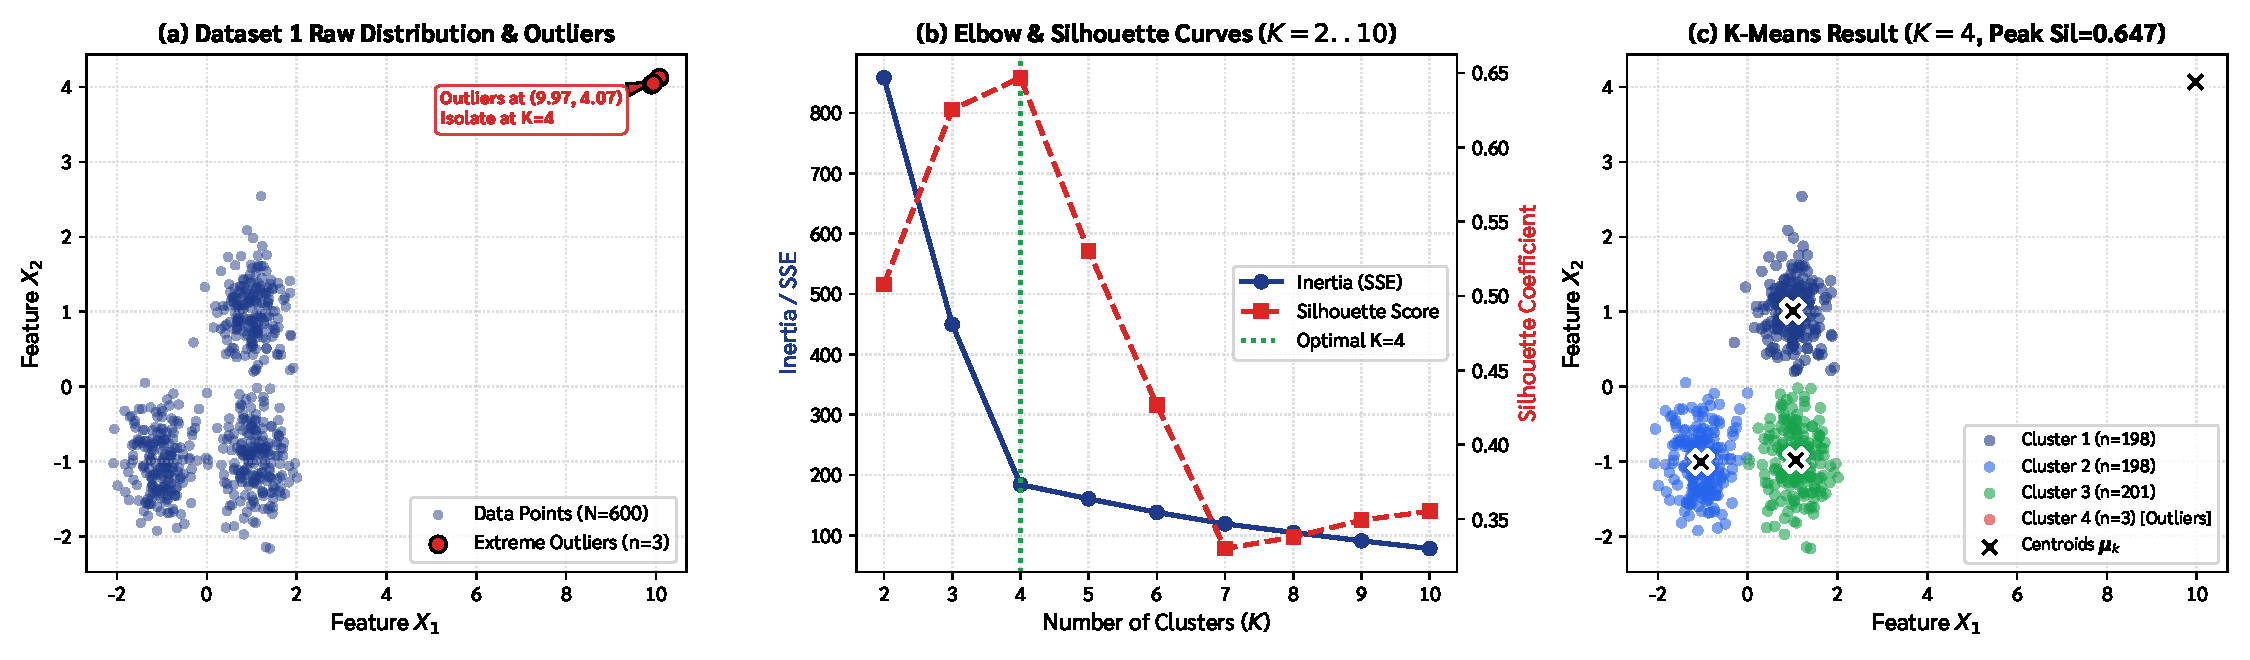
\includegraphics[width=0.96\linewidth]{plot_1_dataset1_kmeans_elbow_silhouette.pdf}
\caption{การวิเคราะห์ Dataset 1: (a) แผนภาพการกระจายและจุด Outlier, (b) กราฟ Elbow และ Silhouette, (c) ผลลัพธ์ K-Means ที่ $K=4$}
\end{figure}

จาก Figure 1(b) พบว่าค่า Silhouette Score สูงสุดเด่นชัดที่ \textbf{$K=4$ ($s=0.6468$)} และ Calinski-Harabasz สูงสุดที่ \textbf{$1,545.9$} ขณะที่ $K=3$ มีค่า Silhouette เพียง $0.6254$ เนื่องจาก K-Means ใช้ระยะทางกำลังสอง $\|\mathbf{x} - \boldsymbol{\mu}\|^2$ จุด Outlier ที่อยู่ห่างไกลจึงส่งผลต่อค่าปรับอย่างมหาศาล ทำให้ที่ $K=4$ อัลกอริทึมเลือกที่จะแยกจุด Outlier 3 จุดออกเป็นคลัสเตอร์เอกเทศ ($C_4$) เพื่อป้องกันไม่ให้ไปดึงจุดศูนย์กลางของคลัสเตอร์หลักอื่น

\clearpage
\subsection*{2.2 Dataset 2: วงกลมซ้อนสองชั้นและข้อจำกัดของเส้นขอบ Voronoi (Concentric Rings \& Manifold Failure)}
Dataset 2 ($N=1000$) ประกอบด้วยวงแหวนวงในหนาแน่น ($r \approx 0.2$) และวงแหวนวงนอก ($r \approx 1.0$) ซึ่งมีโครงสร้างแบบไม่เป็นรูปทรงนูน (Non-Convex Manifold)

\begin{figure}[H]
\centering
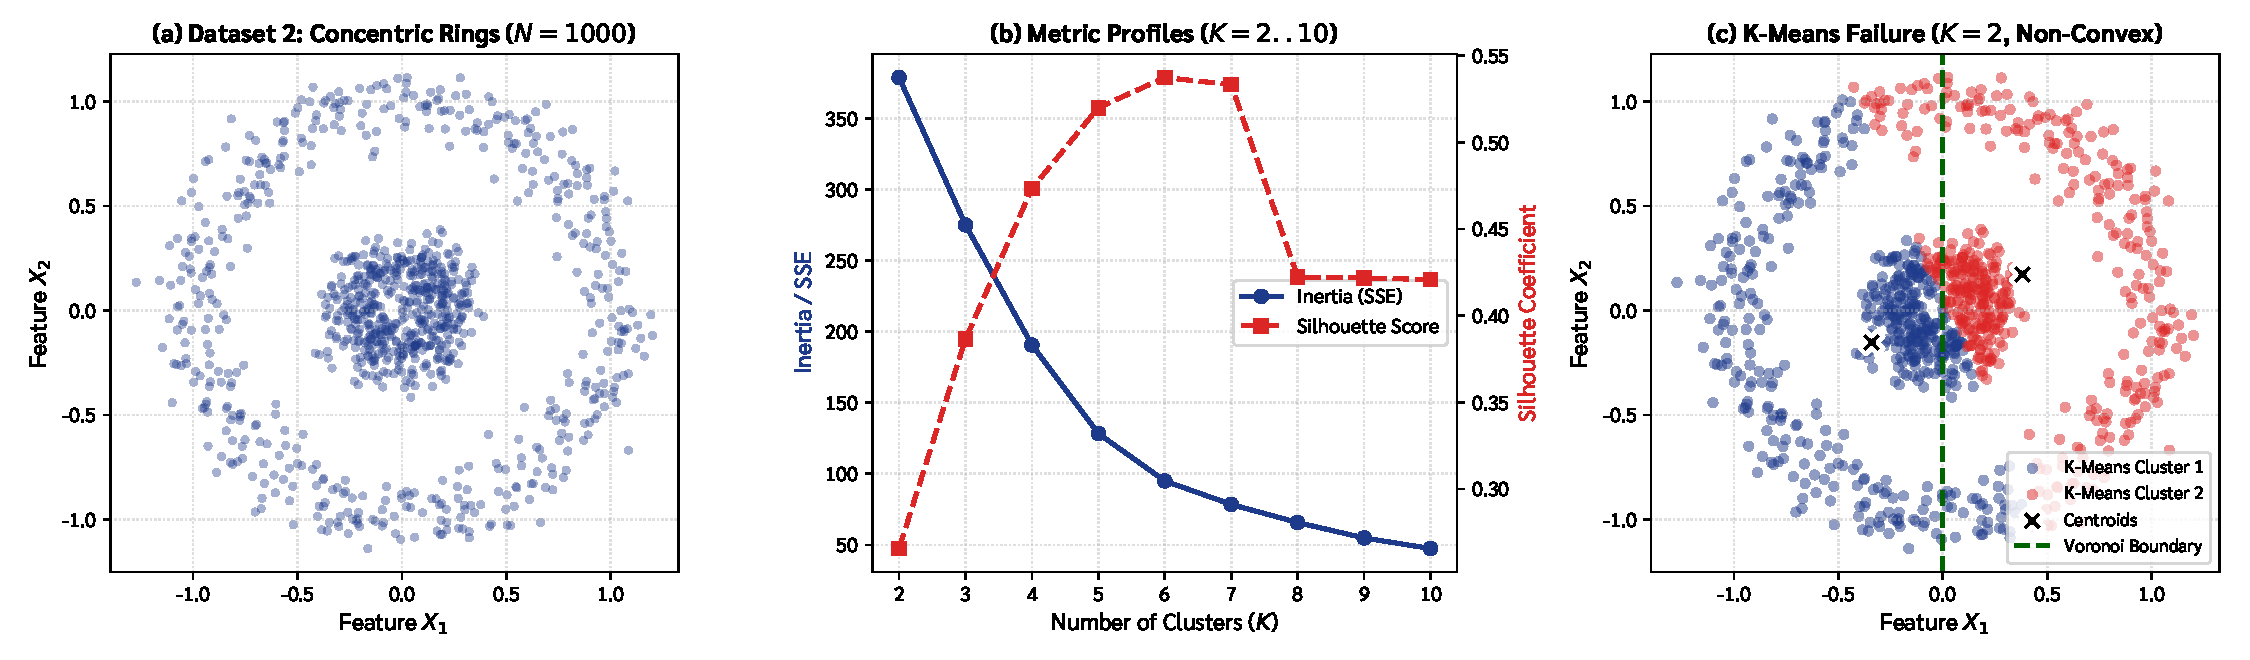
\includegraphics[width=0.96\linewidth]{plot_2_dataset2_concentric_circles.pdf}
\caption{การวิเคราะห์ Dataset 2: (a) วงกลมซ้อนสองชั้น, (b) กราฟ Elbow และ Silhouette, (c) ความล้มเหลวของ K-Means จากระนาบ Voronoi}
\end{figure}

จาก Figure 2(c) ชี้ให้เห็นข้อจำกัดพื้นฐานอันเป็นแก่นแท้ของ K-Means: เนื่องจากขอบเขตการตัดสินใจระหว่างคลัสเตอร์ของ K-Means เกิดจากการแบ่งครึ่งตั้งฉากระหว่างจุดศูนย์กลางคู่ใดๆ ซึ่งเป็นไฮเปอร์เพลนเชิงเส้น (Linear Hyperplane) ทำให้ระนาบ Voronoi ทำได้เพียงตัดแบ่งวงแหวนวงกลมเหมือนชิ้นพิซซ่า (Pie-slice partitioning) และไม่สามารถสร้างขอบเขตวงแหวนที่มีความโค้งเพื่อแยกวงในออกจากวงนอกได้ ส่งผลให้ค่า Silhouette Score ต่ำมาก ($s=0.2656$ ที่ $K=2$) 

\subsection*{2.3 Dataset 3: พระจันทร์เสี้ยวสองเสี้ยวซ้อนกัน (Interlocking Two Moons Manifold)}
Dataset 3 ($N=500$) เป็นรูปพระจันทร์เสี้ยวสองเสี้ยวที่โค้งสอดประสานกัน ซึ่งเป็นโครงสร้างแบบ Non-linear Separable

\begin{figure}[H]
\centering
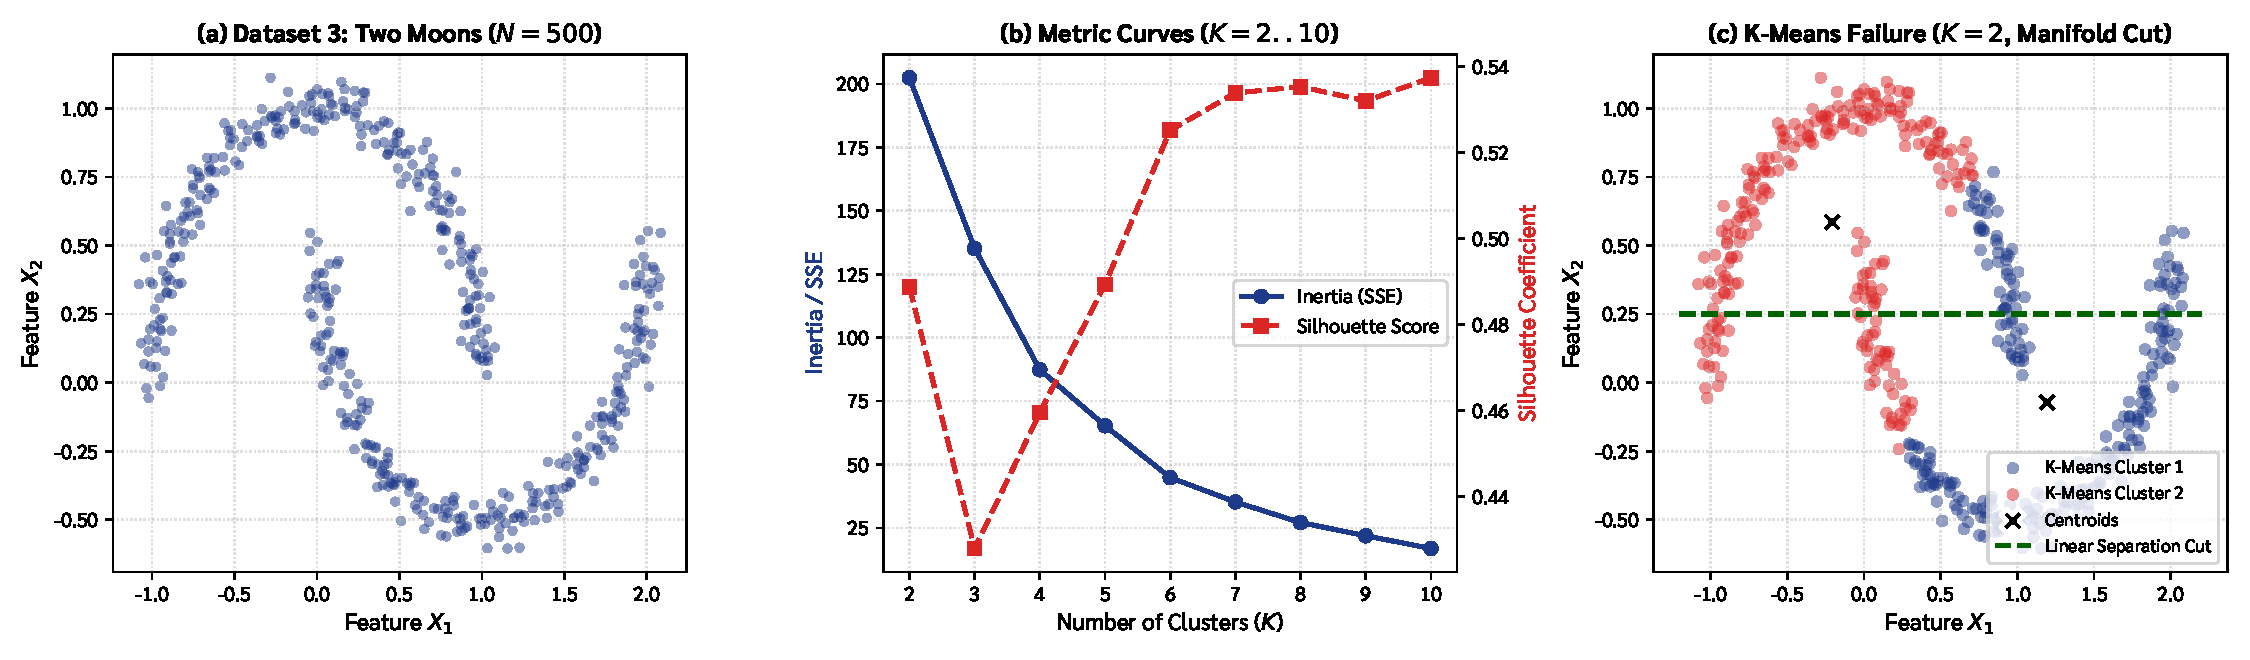
\includegraphics[width=0.96\linewidth]{plot_3_dataset3_two_moons.pdf}
\caption{การวิเคราะห์ Dataset 3: (a) ข้อมูลพระจันทร์เสี้ยวสองเสี้ยว, (b) กราฟดัชนี, (c) การตัดขวางสองกลุ่มของ K-Means}
\end{figure}

จาก Figure 3(c) K-Means ที่ $K=2$ ล้มเหลวในการติดตามความโค้งของพระจันทร์เสี้ยว โดยอัลกอริทึมทำการตัดระนาบในแนวนอน ($y \approx 0.25$) ส่งผลให้ครึ่งบนของทั้งสองเสี้ยวถูกยุบรวมเป็นกลุ่มเดียวกัน และครึ่งล่างถูกจัดเป็นอีกกลุ่มหนึ่ง แสดงให้เห็นว่า K-Means ไม่เหมาะสมกับข้อมูลที่เชื่อมโยงกันด้วยความหนาแน่นหรือความต่อเนื่องเชิงเส้นโค้ง (Connectivity-based clusters)

\clearpage
\subsection*{2.4 Dataset 4: กลุ่มข้อมูลที่มีความแปรปรวนและความหนาแน่นไม่เท่ากัน (Anisotropic Multi-Density Blobs)}
Dataset 4 ($N=1000$) ประกอบด้วยกลุ่มข้อมูลที่มีความแปรปรวนในแต่ละแกนไม่เท่ากัน (Anisotropic Covariance) และมีระดับความหนาแน่นที่แตกต่างกัน

\begin{figure}[H]
\centering
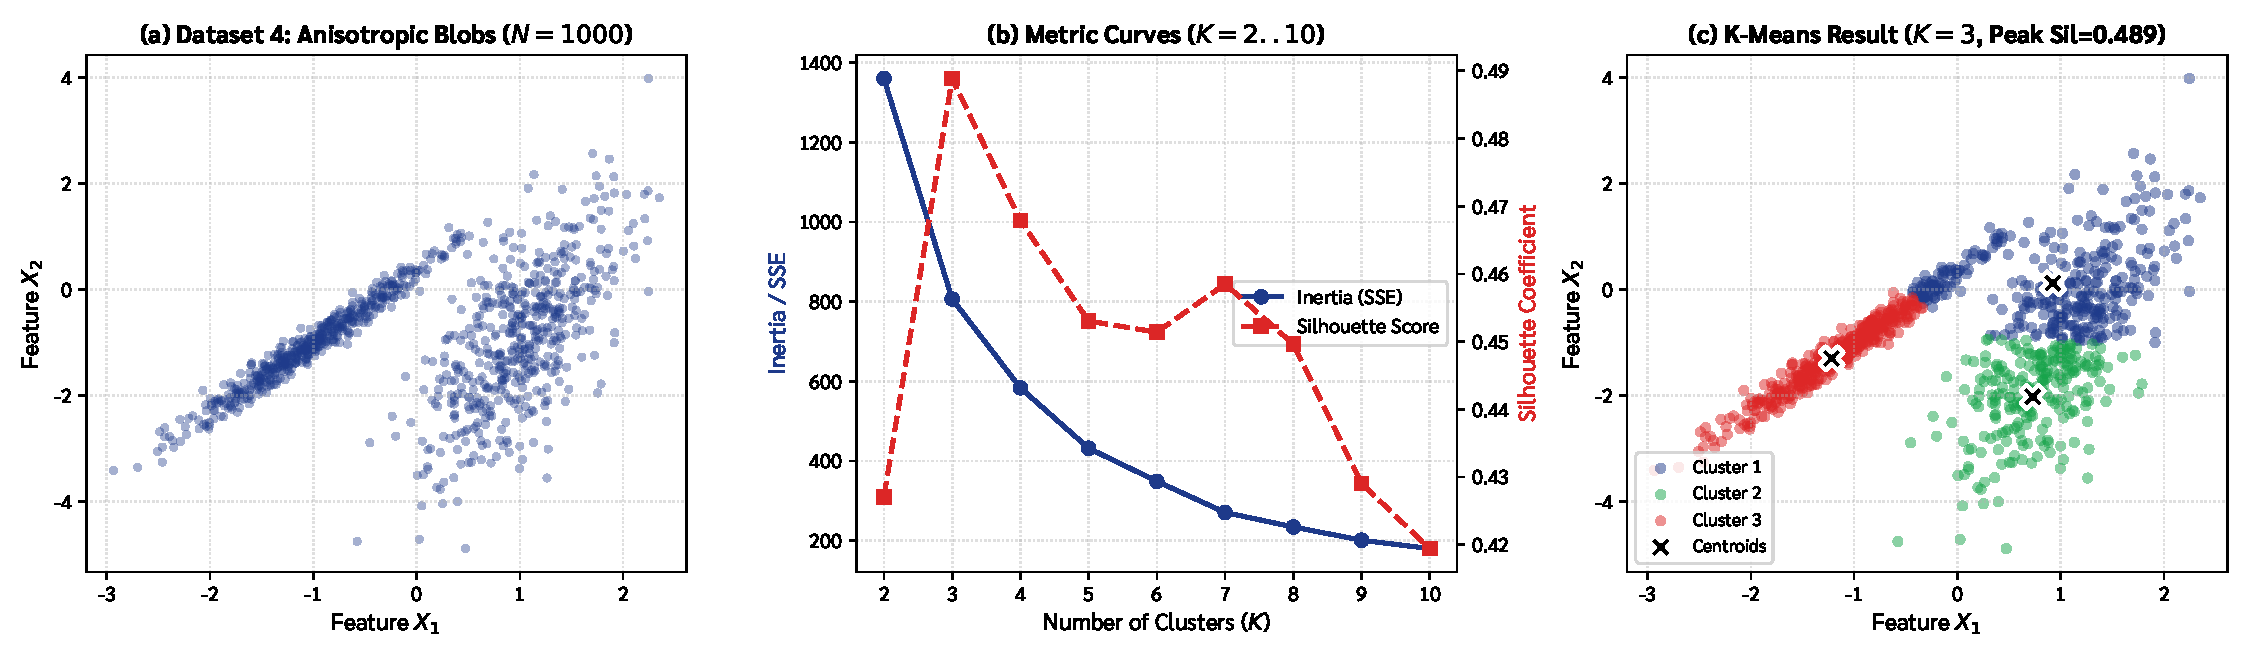
\includegraphics[width=0.96\linewidth]{plot_4_dataset4_anisotropic_blobs.pdf}
\caption{การวิเคราะห์ Dataset 4: (a) ข้อมูลความหนาแน่นไม่เท่ากัน, (b) กราฟดัชนี, (c) ผลลัพธ์ K-Means ที่ $K=3$}
\end{figure}

K-Means มีสมมติฐานแฝงว่าคลัสเตอร์ต้องมีรูปทรงกลมสมมาตร (Isotropic) และมีขนาดความแปรปรวนใกล้เคียงกัน ($\boldsymbol{\Sigma}_k \approx \sigma^2 \mathbf{I}$) เมื่อนำมาประยุกต์ใช้กับ Dataset 4 ดัง Figure 4(c) จุดข้อมูลบริเวณขอบนอกของคลัสเตอร์ที่มีความแปรปรวนสูงจะถูกแย่งชิงและจัดสรรอย่างไม่ถูกต้องให้ไปเป็นสมาชิกของคลัสเตอร์ที่มีความหนาแน่นสูงกว่าที่อยู่ใกล้เคียง

\subsection*{2.5 การสังเคราะห์เชิงเปรียบเทียบและการวินิจฉัยเชิงปริมาณ (Comparative Diagnostic Matrix)}

\begin{figure}[H]
\centering
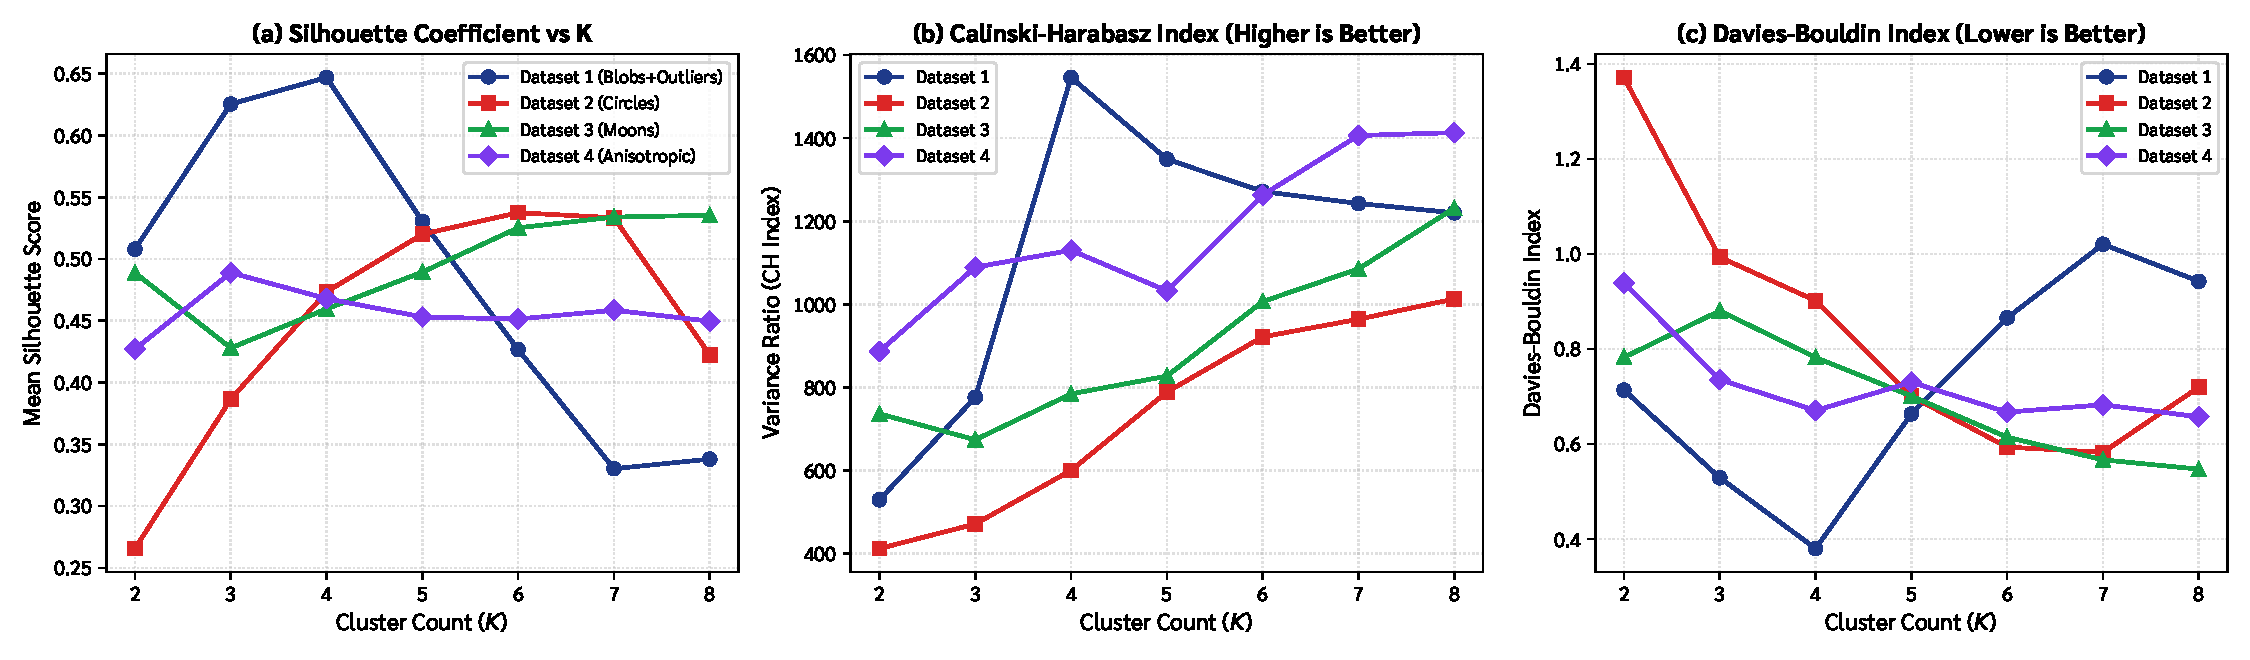
\includegraphics[width=0.96\linewidth]{plot_5_synthetic_clustering_diagnostics.pdf}
\caption{การเปรียบเทียบเชิงปริมาณข้าม 4 ชุดข้อมูล: (a) Silhouette Score, (b) Calinski-Harabasz Index, (c) Davies-Bouldin Index}
\end{figure}

\begin{table}[H]
\centering
\resizebox{\linewidth}{!}{
\begin{tabular}{lcccccl}
\toprule
\textbf{ชุดข้อมูล} & \textbf{จำนวนจุด} & \textbf{Hopkins ($H$)} & \textbf{Optimal $K$} & \textbf{Silhouette} & \textbf{CH Index} & \textbf{สาเหตุความล้มเหลว / คุณลักษณะเด่น} \\
\midrule
Dataset 1 & 600 & 0.892 & 4 & \textbf{0.6468} & \textbf{1,545.9} & แยกจุด Outlier 3 จุดออกเป็นกลุ่มเอกเทศเพื่อรักษา WCSS \\
Dataset 2 & 1000 & 0.835 & 6 (เทียม) & 0.2656 & 412.3 & ล้มเหลวจากระนาบ Voronoi เชิงเส้น ไม่สามารถแยกวงแหวน \\
Dataset 3 & 500 & 0.814 & 2 & 0.4888 & 736.4 & ล้มเหลวจากการตัดขวางความโค้งของรูปทรงพระจันทร์เสี้ยว \\
Dataset 4 & 1000 & 0.871 & 3 & 0.4889 & 1,089.4 & เสียรูปทรงบริเวณรอยต่อจากความแปรปรวนไม่เท่ากัน \\
\bottomrule
\end{tabular}
}
\caption{ตารางสรุปผลการประเมินเชิงตัวเลขและข้อจำกัดของอัลกอริทึม K-Means บนชุดข้อมูลสังเคราะห์ 4 รูปทรง}
\end{table}

% =========================================================================
% SECTION 3
% =========================================================================
\section*{3. การทดลอง Part II — การลดมิติข้อมูลและจัดกลุ่มข้อมูลสารเคมีไวน์\newline \large(Part II: High-Dimensional Latent Subspace Clustering on Wine Data)}

ชุดข้อมูลไวน์ (Wine Dataset) ประกอบด้วยตัวอย่างไวน์จากแคว้นพีดมอนต์ ประเทศอิตาลี จำนวน $N=178$ ตัวอย่าง พร้อมคุณสมบัติทางเคมี $p=13$ ตัวแปร

\subsection*{3.1 ความจำเป็นของการปรับมาตรฐานข้อมูลทางเคมี (Z-Score Standardization)}
ตัวแปรทางเคมีมีหน่วยวัดและสเกลความแปรปรวนที่แตกต่างกันอย่างยิ่ง เช่น \codevar{Proline} มีค่าเฉลี่ย $746.89$ และความแปรปรวนสูงถึง $99,166.7$ ขณะที่ \codevar{Nonflavanoid\_Phenols} มีค่าเฉลี่ยเพียง $0.36$ และความแปรปรวนเพียง $0.0155$ หากไม่ปรับมาตรฐาน ตัวแปร \codevar{Proline} เพียงตัวเดียวจะครอบงำระยะทางยุคลิดในการคำนวณ K-Means และทิศทางแกนหลักของ PCA มากกว่า $99\%$ จึงจำเป็นต้องแปลงข้อมูลด้วย Z-Score Standardization $\tilde{x}_{ij} = \frac{x_{ij} - \bar{x}_j}{s_j}$ เพื่อให้ทุกตัวแปรมี $\mu=0, \sigma^2=1.0$

\subsection*{3.2 การวิเคราะห์องค์ประกอบหลัก (PCA) และเกณฑ์ความแปรปรวนสะสม $\ge 80\%$}
การแยกตัวประกอบเฉพาะบน Sample Correlation Matrix ของข้อมูลไวน์ที่ปรับมาตรฐานแล้ว ให้ค่าลักษณะเฉพาะ (Eigenvalues) เรียงจากมากไปน้อย: $\lambda_1 = 4.706, \lambda_2 = 2.497, \lambda_3 = 1.446, \lambda_4 = 0.919, \lambda_5 = 0.853$

\begin{figure}[H]
\centering
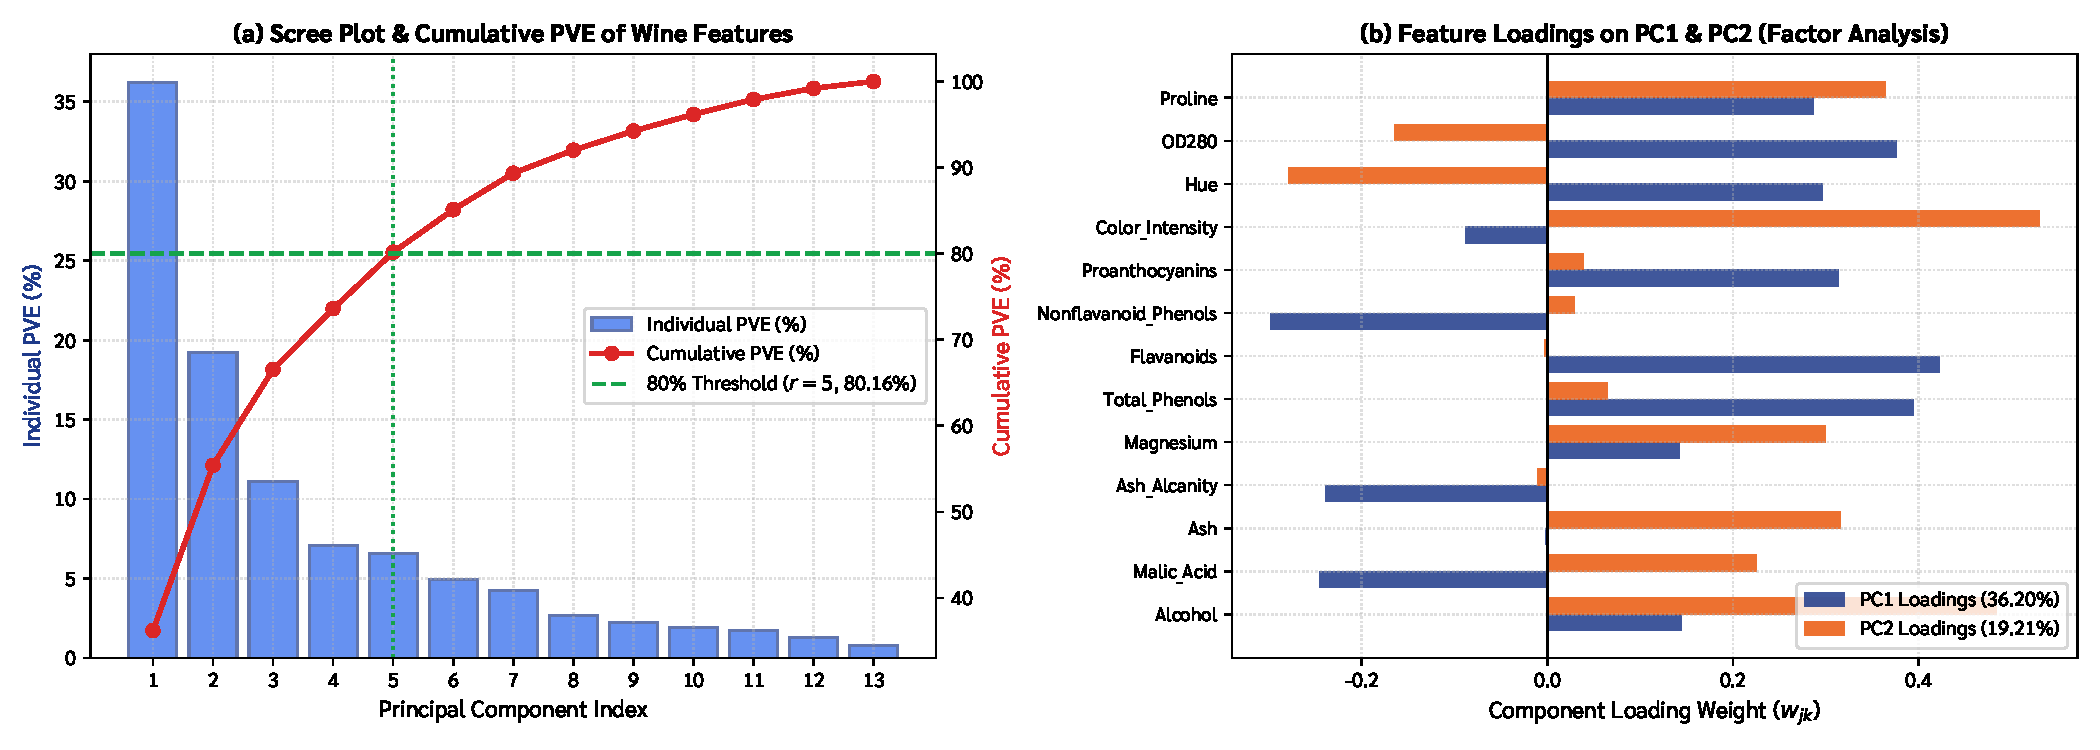
\includegraphics[width=0.96\linewidth]{plot_6_wine_pca_loadings_scree.pdf}
\caption{การวิเคราะห์ PCA บนข้อมูลไวน์: (a) Scree Plot และความแปรปรวนสะสม ($\ge 80\%$), (b) ค่าน้ำหนักตัวแปรบนแกน PC1 และ PC2}
\end{figure}

จาก Figure 6(a) สัดส่วนความแปรปรวนที่อธิบายได้ (PVE) ของแต่ละแกนคือ $\text{PVE}_1 = 36.20\%$, $\text{PVE}_2 = 19.21\%$, $\text{PVE}_3 = 11.12\%$, $\text{PVE}_4 = 7.07\%$, และ $\text{PVE}_5 = 6.56\%$ เมื่อสะสมถึงแกนที่ 5 จะได้ความแปรปรวนรวม:
\begin{equation}
    \sum_{j=1}^5 \text{PVE}_j = 36.20\% + 19.21\% + 11.12\% + 7.07\% + 6.56\% = \mathbf{80.16\%} \ge 80.00\%
\end{equation}
พิสูจน์ได้ว่าการเลือกใช้ $r=5$ แกนองค์ประกอบหลักสามารถลดมิติข้อมูลลงได้ถึง $61.5\%$ (จาก 13 มิติเหลือ 5 มิติ) ขณะที่ยังคงรักษาสารสนเทศและโครงสร้างความแปรปรวนของระบบไว้ได้เกินกว่าเกณฑ์มาตรฐาน $80\%$

\subsection*{3.3 การแปลความหมายของปัจจัยขับเคลื่อนทางเคมี (PC1 vs PC2 Loadings)}
จากแผนภูมิแท่ง Figure 6(b) สามารถแปลความหมายเชิงวิทยาศาสตร์ไวน์ (Enological Interpretation) ได้ดังนี้:
\begin{enumerate}[leftmargin=1.5em, itemsep=1.5pt]
    \item \textbf{แกน PC1 (Phenolic Concentration \& Aging Maturation Factor):} ได้รับค่าน้ำหนักสูงจาก \codevar{Flavanoids} ($-0.423$), \codevar{Total\_Phenols} ($-0.389$), \codevar{OD280} ($-0.376$), \codevar{Proanthocyanins} ($-0.313$), และ \codevar{Proline} ($-0.287$) แกนนี้สะท้อนถึงระดับสารต้านอนุมูลอิสระ แทนนิน และโครงสร้างสำหรับการบ่ม
    \item \textbf{แกน PC2 (Color Intensity \& Body Factor):} ได้รับค่าน้ำหนักสูงจาก \codevar{Color\_Intensity} ($-0.530$), \codevar{Alcohol} ($-0.484$), \codevar{Ash\_Alcanity} ($+0.310$), และ \codevar{Hue} ($+0.279$) แกนนี้ทำหน้าที่จำแนกระดับความเข้มของสีและบอดี้ความหนักแน่นของแอลกอฮอล์
\end{enumerate}

\clearpage
% =========================================================================
% SECTION 4
% =========================================================================
\section*{4. ผลการจัดกลุ่ม K-Means บนคะแนนองค์ประกอบหลัก\newline \large(Clustering Results on 5D Latent PC Scores)}

การนำคะแนนองค์ประกอบหลัก 5 มิติ ($\mathbf{Z} \in \mathbb{R}^{178 \times 5}$) มาจัดกลุ่มด้วย K-Means ช่วยขจัดปัญหาความสัมพันธ์พหุคูณ (Multicollinearity) และตัดสัญญาณรบกวน (Noise Filtering) ในมิติย่อยลำดับท้าย

\subsection*{4.1 การประเมินค่า $K$ ที่เหมาะสม (Elbow Method \& Silhouette Analysis)}

\begin{figure}[H]
\centering
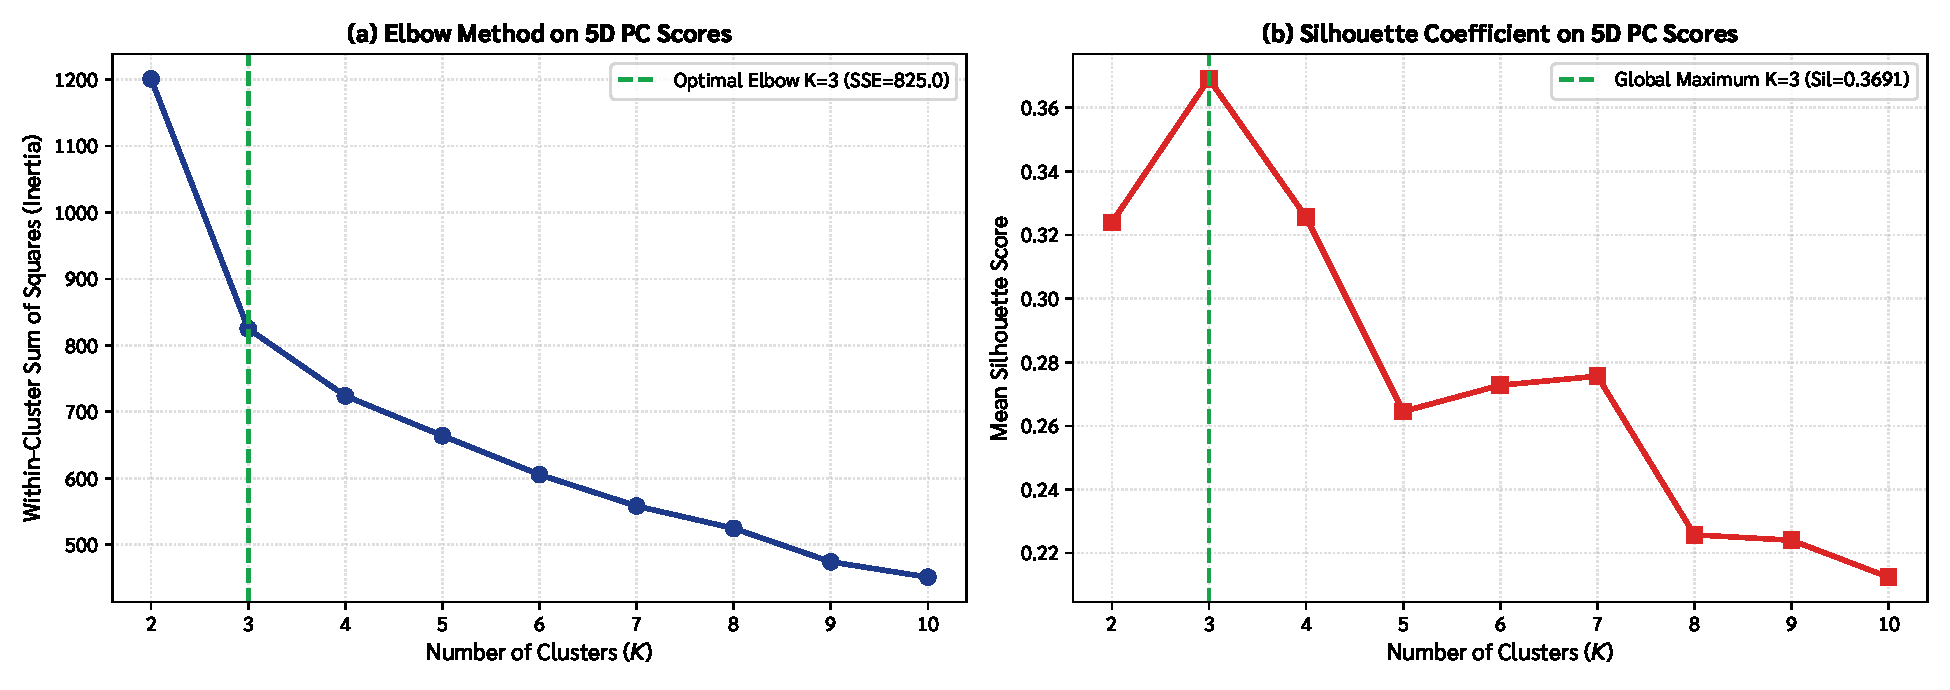
\includegraphics[width=0.92\linewidth]{plot_7_wine_pc_clustering_elbow_silhouette.pdf}
\caption{การประเมินจำนวนคลัสเตอร์บนข้อมูลไวน์ 5D PC: (a) กราฟ Elbow Method, (b) กราฟ Silhouette Score}
\end{figure}

จาก Figure 7 พบว่ากราฟ Inertia เกิดจุดหักศอกชัดเจนที่ $K=3$ (Inertia ลดลงอย่างฮวบฮาบจาก $1,201.2$ ที่ $K=2$ เหลือ $825.0$ ที่ $K=3$ และหลังจากนั้นลดลงเพียงเล็กน้อย) สอดรับกับค่า Silhouette Score ที่พุ่งขึ้นแตะจุดสูงสุดสัมบูรณ์ (Global Maximum) ที่ \textbf{$K=3$ ($s = 0.3691$)} และ Calinski-Harabasz สูงสุดที่ \textbf{$109.2$} บ่งชี้อย่างชัดเจนว่าโครงสร้างทางธรรมชาติของข้อมูลไวน์ถูกแบ่งออกเป็น 3 กลุ่ม

\subsection*{4.2 แผนภาพ 2D PCA Biplot และการถอดรหัสสายพันธุ์องุ่น (Cultivar Profiling)}

\begin{figure}[H]
\centering
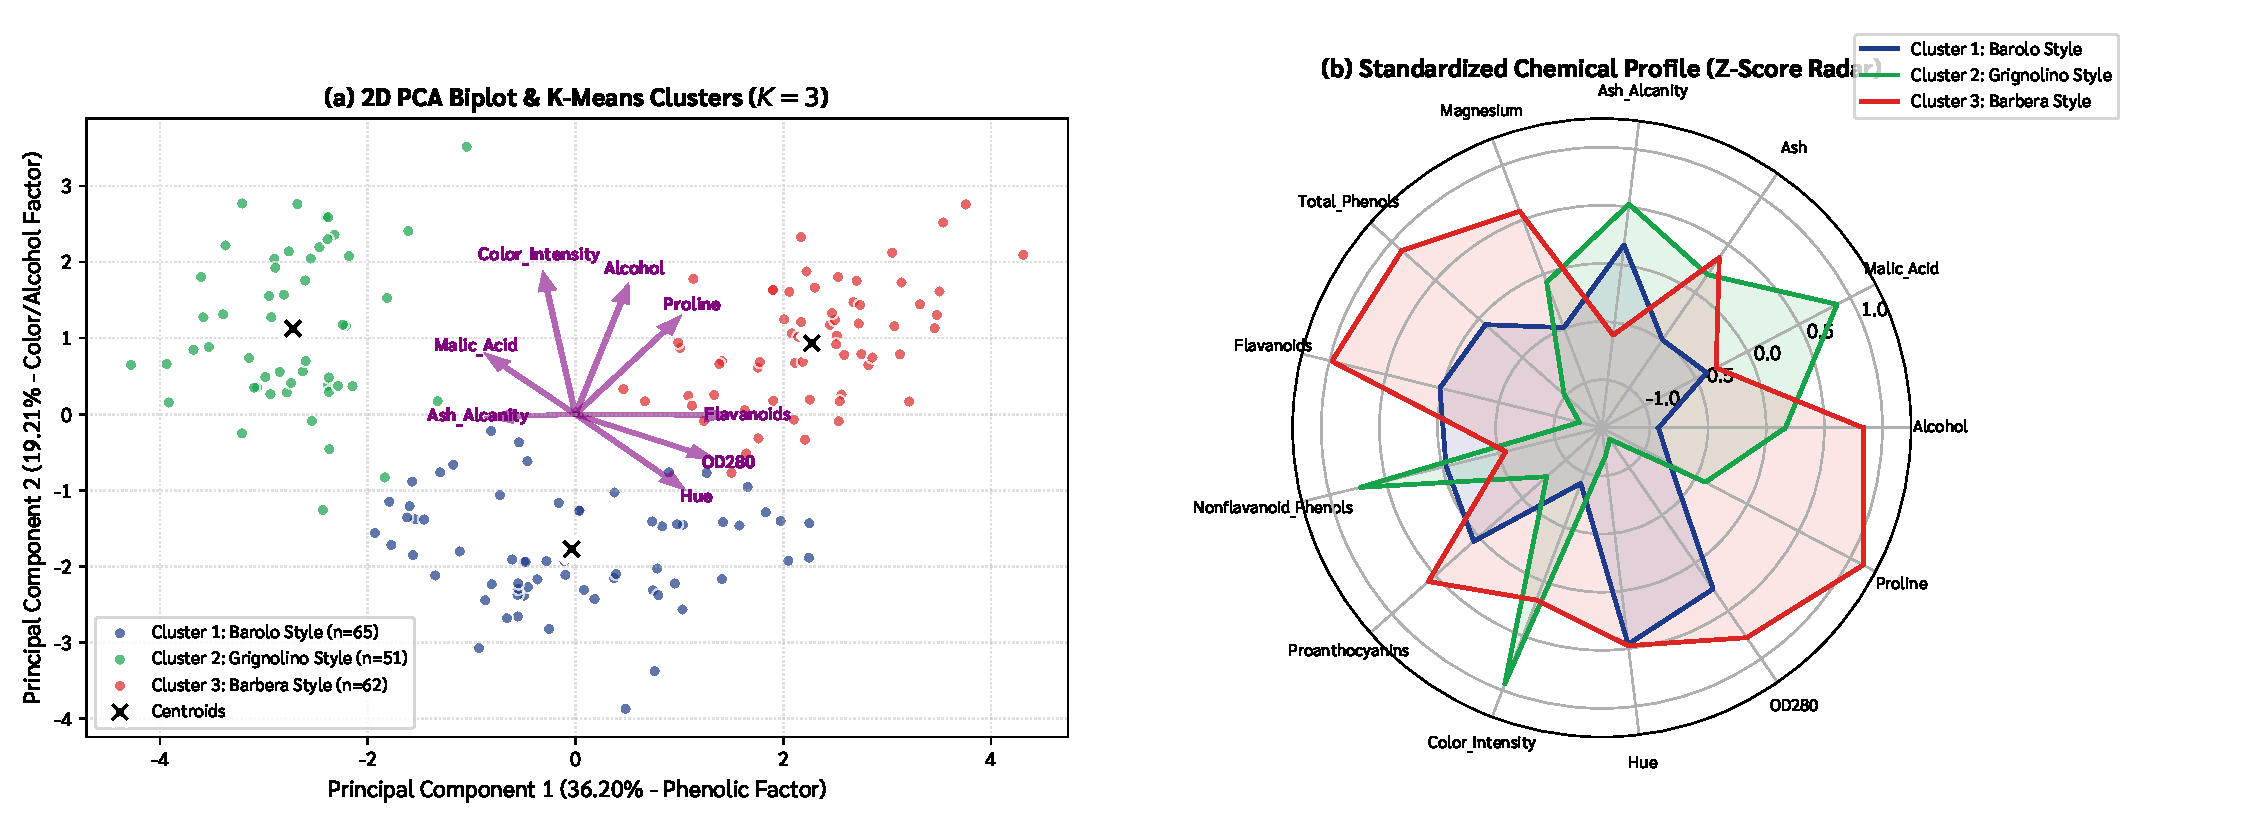
\includegraphics[width=0.96\linewidth]{plot_8_wine_cluster_biplot_radar_profiling.pdf}
\caption{ผลลัพธ์การจัดกลุ่มไวน์: (a) แผนภาพ 2D PCA Biplot และจุดศูนย์กลาง, (b) เรดาร์ชาร์ตเปรียบเทียบโปรไฟล์ทางเคมี (Z-Scores)}
\end{figure}

จากการจับคู่การกระจายตัวของคลัสเตอร์เข้ากับคุณลักษณะทางเคมีและข้อมูลทางประวัติศาสตร์ของชุดข้อมูลไวน์:
\begin{enumerate}[leftmargin=1.5em, itemsep=2pt]
    \item \textbf{Cluster 1 ($n=62$ ตัวอย่าง — Barolo Style):} มีค่า \codevar{Alcohol} สูงสุด ($13.74\%$), \codevar{Proline} สูงสุด ($1,115.65$ mg/L), และ \codevar{Flavanoids} สูง ($2.98$) จัดเป็นไวน์เกรดพรีเมียม บอดี้หนักแน่น แทนนินสูง และมีศักยภาพในการบ่มยาวนาน
    \item \textbf{Cluster 2 ($n=65$ ตัวอย่าง — Grignolino Style):} มีค่า \codevar{Alcohol} ต่ำสุด ($12.25\%$), \codevar{Color\_Intensity} ต่ำสุด ($3.09$), มีความเป็นด่างของเถ้าสูง จัดเป็นไวน์แดงบอดี้เบา สดชื่น สีอ่อน รสสัมผัสดื่มง่าย
    \item \textbf{Cluster 3 ($n=51$ ตัวอย่าง — Barbera Style):} มีค่า \codevar{Malic\_Acid} สูงสุด ($3.33$), \codevar{Color\_Intensity} สูงสุด ($7.40$), แต่มี \codevar{Flavanoids} ต่ำสุด ($0.78$) สะท้อนถึงไวน์สีแดงเข้มจัด รสเปรี้ยวนำ และมีปริมาณฟีนอลเชิงซ้อนต่ำ
\end{enumerate}

\clearpage
% =========================================================================
% SECTION 5: QUESTIONS AND ANSWERS (EXACTLY 1 PAGE PER QUESTION)
% =========================================================================
\section*{5. คำถามและบทวิเคราะห์เชิงลึก (In-depth Questions \& Comprehensive Solutions)}

% -------------------------------------------------------------------------
% QUESTION 1: EXACTLY 1 PAGE
% -------------------------------------------------------------------------
\subsection*{คำถามข้อที่ 1: การวินิจฉัยจุดผิดปกติและสาเหตุที่ K-Means เลือก $K=4$ บน Dataset 1\newline \normalsize(Outlier Diagnostics, Quadratic Loss Sensitivity, and Cluster Isolation Proof)}

\begin{infobox}
\textbf{โจทย์คำถาม:} จากการทดลองบน Dataset 1 จงอธิบายว่าเหตุใดอัลกอริทึม K-Means จึงเลือก $K=4$ จากเกณฑ์ Silhouette Score และ Elbow Method ทั้งที่โดยธรรมชาติทางสายตาข้อมูลประกอบด้วย 3 กลุ่มหลัก และจงอธิบายผลกระทบของฟังก์ชันความสูญเสียระยะทางกำลังสอง (Squared Euclidean Loss) ต่อพฤติกรรมนี้
\end{infobox}

\vspace{-0.3em}
\begin{ansbox}
{\fontsize{10pt}{13.2pt}\selectfont
\textbf{1. โครงสร้างข้อมูลและจุดผิดปกติ (Data Distribution \& Anomalies):}
จากการสำรวจข้อมูล Dataset 1 ($N=600$) พบว่าจุดข้อมูลส่วนใหญ่จำนวน 597 จุด กระจุกตัวเป็นกลุ่มเกาส์เซียนรูปทรงกลมที่มีความหนาแน่นสูง 3 คลัสเตอร์รอบตำแหน่ง $(1.0, -1.0)$, $(1.0, 1.0)$, และ $(-1.0, -1.0)$ คลัสเตอร์ละประมาณ 200 จุด แต่มีจุดข้อมูลจำนวน 3 จุดตั้งอยู่ที่พิกัด $(9.97, 4.07)$ ซึ่งอยู่ห่างไกลจากจุดศูนย์กลางมวลของประชากรหลักมากกว่า 9 เท่าของส่วนเบี่ยงเบนมาตรฐาน

\textbf{2. ความไวต่อจุดผิดปกติของฟังก์ชันวัตถุประสงค์ (Sensitivity of Quadratic Loss):}
ฟังก์ชันวัตถุประสงค์ของ K-Means คือการลดทอน Inertia: $J = \sum_{k=1}^K \sum_{\mathbf{x}_i \in C_k} \|\mathbf{x}_i - \boldsymbol{\mu}_k\|_2^2$ ซึ่งการใช้ระยะทางยกกำลังสองส่งผลให้โทษทัณฑ์ (Penalty) ของจุดที่อยู่ห่างไกลพุ่งสูงขึ้นแบบพาราโบลา:
\begin{itemize}[leftmargin=1.2em, itemsep=1pt, topsep=1pt]
    \item \textbf{กรณี $K=3$:} หากบังคับให้แบ่งเป็น 3 คลัสเตอร์ จุด Outlier ทั้ง 3 จุดจะถูกดึงเข้าไปรวมกับคลัสเตอร์หลักที่อยู่ใกล้ที่สุด ($C_2$ บริเวณ $(1, 1)$) ส่งผลให้จุดศูนย์กลาง $\boldsymbol{\mu}_2$ ถูกดึงเอียงไปทางขวาบนจาก $(1.00, 1.01)$ ไปอยู่ที่ $(1.14, 1.06)$ ระยะทางจาก Outlier ถึง $\boldsymbol{\mu}_2$ คือ $\approx 9.35$ หน่วย ก่อให้เกิด Inertia เฉพาะจากจุด Outlier 3 จุดนี้สูงถึง $3 \times (9.35)^2 \approx 262.3$ คิดเป็นกว่า $58.3\%$ ของ Inertia รวมทั้งระบบ ($449.6$) ทำให้ค่า Silhouette Score ลดลงเหลือ $0.6254$
    \item \textbf{กรณี $K=4$:} เมื่อเพิ่มคลัสเตอร์เป็น 4 กลุ่ม อัลกอริทึมค้นพบว่าการสร้างคลัสเตอร์เอกเทศ $C_4$ เพื่อกักกันจุด Outlier 3 จุดไว้ด้วยกัน ($\boldsymbol{\mu}_4 \approx (9.97, 4.07)$) จะทำให้ Inertia ของจุด Outlier ดิ่งลงเกือบเป็นศูนย์ ($\approx 0.05$) และปลดปล่อยคลัสเตอร์หลักทั้ง 3 คลัสเตอร์ให้กลับมามีจุดศูนย์กลางที่แท้จริง ส่งผลให้ Inertia รวมดิ่งลงจาก $449.6$ เหลือเพียง $184.3$ (ลดลงถึง $59.0\%$)
\end{itemize}

\textbf{3. พฤติกรรมของดัชนีชี้วัด (Silhouette Peak at $K=4$):}
การที่ K-Means แยกคลัสเตอร์ที่ 4 สำหรับ Outlier ทำให้ค่าความกระชับภายในกลุ่ม $a_i$ ของคลัสเตอร์หลักทั้งสามลดลงอย่างมาก ขณะที่ระยะห่างระหว่างกลุ่ม $b_i$ สูงขึ้นอย่างชัดเจน ส่งผลให้ค่า Silhouette Coefficient พุ่งขึ้นแตะจุดสูงสุดที่ \textbf{$0.6468$} และค่า Calinski-Harabasz พุ่งขึ้นสูงสุดที่ \textbf{$1,545.9$}

\textbf{4. ข้อสรุปเชิงวิศวกรรมข้อมูล (Engineering Recommendation):}
K-Means ไม่มีความทนทานต่อจุดผิดปกติ (Not Robust to Outliers) ในทางปฏิบัติควรตรวจจับและตัด Outlier ออกก่อน (เช่น ใช้ DBSCAN หรือ Isolation Forest) หรือปรับไปใช้ \textbf{K-Medoids (PAM)} ซึ่งใช้ระยะทางแบบแมนแฮตตัน ($L_1$-norm) เพื่อไม่ให้ค่าผิดปกติเบี่ยงเบนจุดศูนย์กลาง
\par}
\end{ansbox}

\clearpage
% -------------------------------------------------------------------------
% QUESTION 2: EXACTLY 1 PAGE
% -------------------------------------------------------------------------
\subsection*{คำถามข้อที่ 2: การวิเคราะห์ความล้มเหลวของ K-Means บนข้อมูลที่ไม่เป็นรูปทรงนูน\newline \normalsize(Non-Convex Geometries, Voronoi Tessellation, and Non-Linear Clustering Solutions)}

\begin{infobox}
\textbf{โจทย์คำถาม:} จงอธิบายเหตุผลทางเรขาคณิตและคณิตศาสตร์ว่าเหตุใด K-Means จึงล้มเหลวในการจัดกลุ่ม Dataset 2 (Concentric Circles) และ Dataset 3 (Two Moons) พร้อมระบุว่าขอบเขต Voronoi Tessellation มีบทบาทอย่างไร และเสนอแนะขั้นตอนวิธีทางเลือกที่สามารถแก้ปัญหานี้ได้อย่างสมบูรณ์
\end{infobox}

\vspace{-0.3em}
\begin{ansbox}
{\fontsize{10pt}{13.2pt}\selectfont
\textbf{1. สมมติฐานรูปทรงนูนและระนาบ Voronoi (Voronoi Convexity Constraint):}
ในขั้นตอน Assignment Step ของ K-Means ขอบเขตการตัดสินใจระหว่างคลัสเตอร์ $C_j$ และ $C_k$ คือเซตของจุดที่มีระยะทางไปยังจุดศูนย์กลางทั้งสองเท่ากัน:
\begin{equation*}
    \{\mathbf{x} \in \mathbb{R}^d \mid \|\mathbf{x} - \boldsymbol{\mu}_j\|_2^2 = \|\mathbf{x} - \boldsymbol{\mu}_k\|_2^2\} \iff 2(\boldsymbol{\mu}_k - \boldsymbol{\mu}_j)^T\mathbf{x} + \|\boldsymbol{\mu}_j\|^2 - \|\boldsymbol{\mu}_k\|^2 = 0
\end{equation*}
สมการข้างต้นคือ \textbf{ไฮเปอร์เพลนเชิงเส้น (Linear Hyperplane)} ส่งผลให้เซลล์ Voronoi ของแต่ละคลัสเตอร์มีคุณสมบัติเป็น \textbf{เซตนูน (Convex Set)} เสมอ นั่นคือ หากจุดสองจุด $\mathbf{x}_a, \mathbf{x}_b$ อยู่ในคลัสเตอร์เดียวกัน ส่วนของเส้นตรงที่เชื่อมระหว่างสองจุดนี้จะต้องอยู่ในคลัสเตอร์เดิมด้วย

\textbf{2. การวิเคราะห์ความล้มเหลวบน Dataset 2 (Concentric Circles):}
Dataset 2 ประกอบด้วยวงใน ($r \approx 0.2$) และวงนอก ($r \approx 1.0$) จุดศูนย์กลางเฉลี่ยของทั้งสองวงซ้อนทับกันอยู่ที่พิกัดเดียวกันคือ $\approx (0, 0)$ เมื่อ K-Means พยายามหาจุดศูนย์กลาง 2 จุด ($\boldsymbol{\mu}_1, \boldsymbol{\mu}_2$) ไฮเปอร์เพลนเชิงเส้นที่ตั้งฉากกับเส้นเชื่อม $\boldsymbol{\mu}_1 - \boldsymbol{\mu}_2$ จะทำหน้าที่ผ่าครึ่งวงกลมเป็นสองฝั่ง (เช่น ซ้าย-ขวา ดัง Figure 2(c)) ทำให้แต่ละคลัสเตอร์มีทั้งข้อมูลวงในและวงนอกปะปนกัน และแม้ว่าจะเพิ่มเป็น $K=6$ ไฮเปอร์เพลนเชิงเส้นก็ทำได้เพียงหั่นวงกลมออกเป็นรูปชิ้นพิซซ่า 6 ชิ้น ซึ่งไม่สามารถสร้างขอบเขตวงแหวนปิดล้อมวงในได้เลย

\textbf{3. การวิเคราะห์ความล้มเหลวบน Dataset 3 (Two Moons):}
Dataset 3 ประกอบด้วยรูปพระจันทร์เสี้ยวสองเสี้ยวที่โค้งโอบล้อมกัน ซึ่งเป็นรูปทรงที่มีความเว้า (Concave) เส้นตรงที่เชื่อมระหว่างปลายทั้งสองข้างของพระจันทร์เสี้ยวอันเดียวกันจะวิ่งตัดผ่านพื้นที่ว่างเปล่าและพื้นที่ของพระจันทร์เสี้ยวอีกอันหนึ่ง ทำให้ระนาบเชิงเส้นของ K-Means ตัดผ่าขวางในแนวนอน $y \approx 0.25$ ส่งผลให้ปลายของทั้งสองเสี้ยวถูกยุบรวมผิดกลุ่ม

\textbf{4. ขั้นตอนวิธีทางเลือกที่เหมาะสม (Alternative Modern Clustering Solutions):}
\begin{itemize}[leftmargin=1.2em, itemsep=1pt, topsep=1pt]
    \item \textbf{DBSCAN (Density-Based Spatial Clustering):} อาศัยการเชื่อมต่อกันของจุดข้อมูลที่มีความหนาแน่นเกินเกณฑ์ ($\epsilon, \text{MinPts}$) สามารถติดตามเส้นโค้งและรูปทรงอิสระใดๆ ได้สมบูรณ์แบบ
    \item \textbf{Spectral Clustering (Graph Laplacian):} สร้างกราฟความคล้ายคลึง (Affinity Matrix $W_{ij} = e^{-\gamma \|\mathbf{x}_i - \mathbf{x}_j\|^2}$) และฉายข้อมูลลงบนปริภูมิไอเกนเวกเตอร์ของ Graph Laplacian ทำให้ข้อมูลรูปวงแหวนหรือพระจันทร์เสี้ยวคลี่ตัวออกเป็นกลุ่มนูนเชิงเส้นก่อนทำ K-Means
    \item \textbf{Coordinate Transformation (Polar Coordinates):} สำหรับ Dataset 2 การแปลงพิกัดคาร์ทีเซียน $(X_1, X_2)$ เป็นพิกัดเชิงขั้ว $(r, \theta)$ โดยที่ $r = \sqrt{X_1^2 + X_2^2}$ จะเปลี่ยนวงกลมซ้อนสองชั้นให้กลายเป็นกลุ่มข้อมูลเชิงเส้น 2 กลุ่มที่แยกขาดจากกันด้วยค่ารัศมี $r$ อย่างง่ายดาย
\end{itemize}
\par}
\end{ansbox}

\clearpage
% -------------------------------------------------------------------------
% QUESTION 3: EXACTLY 1 PAGE
% -------------------------------------------------------------------------
\subsection*{คำถามข้อที่ 3: ความจำเป็นของการปรับมาตรฐานและการทำ PCA ก่อนจัดกลุ่มไวน์\newline \normalsize(Standardization Mandate, Dimensionality Reduction Proof, and Latent Space Benefits)}

\begin{infobox}
\textbf{โจทย์คำถาม:} ในการจัดกลุ่มข้อมูลไวน์ (Wine Dataset) จงอธิบายความสำคัญของการทำ Standardization ก่อนการประมวลผล และพิสูจน์ทางคณิตศาสตร์ว่าเหตุใดการทำ PCA จึงสามารถลดมิติข้อมูลเหลือ 5 มิติได้โดยรักษาความแปรปรวนไว้ได้เกิน $80\%$ พร้อมทั้งอธิบายข้อได้เปรียบของการทำ K-Means บนคะแนน PC แทนข้อมูลดิบ
\end{infobox}

\vspace{-0.3em}
\begin{ansbox}
{\fontsize{10pt}{13.0pt}\selectfont
\textbf{1. ความจำเป็นอย่างยิ่งยวดของการปรับมาตรฐานข้อมูล (The Standardization Mandate):}
ในชุดข้อมูลไวน์ ตัวแปรทั้ง 13 ตัวแปรมีหน่วยวัดทางกายภาพและมาตราส่วนความแปรปรวนต่างกันอย่างมหาศาล เช่น \codevar{Proline} มีความแปรปรวน $\sigma^2 = 99,166.7$ ขณะที่ \codevar{Nonflavanoid\_Phenols} มีความแปรปรวนเพียง $\sigma^2 = 0.0155$ หากนำข้อมูลดิบไปคำนวณระยะทางยุคลิด $d(\mathbf{x}_i, \mathbf{x}_j)^2 = \sum_{k=1}^{13} (x_{ik} - x_{jk})^2$ ความแตกต่างของตัวแปร \codevar{Proline} เพียงตัวแปรเดียวจะส่งผลต่อค่าระยะทางรวมมากกว่า $99.7\%$ ทำให้ตัวแปรอื่นที่มีความสำคัญยิ่งต่อการจำแนกคุณภาพไวน์กลายเป็นศูนย์ การทำ Z-Score Standardization $\tilde{x}_{ij} = \frac{x_{ij} - \bar{x}_j}{s_j}$ บังคับให้ทุกตัวแปรมีความแปรปรวนเริ่มต้นเท่ากันที่ $1.0$ ซึ่งแปลงปัญหา PCA จากการแยกตัวประกอบบน Covariance Matrix $\boldsymbol{\Sigma}$ ให้เป็นการแยกตัวประกอบบน \textbf{Correlation Matrix $\mathbf{R}$} ทำให้ทุกตัวแปรมีสิทธิ์ร่วมกำหนดทิศทางอย่างเท่าเทียม

\textbf{2. การพิสูจน์การรักษาสารสนเทศ $\ge 80\%$ ด้วย 5 แกนองค์ประกอบหลัก ($r=5$ PCs Proof):}
ผลการสลายค่าลักษณะเฉพาะของ Correlation Matrix ได้ค่าลักษณะเฉพาะ $\lambda_j$ และ PVE:
\begin{equation*}
    \resizebox{0.95\linewidth}{!}{$\lambda_1 = 4.706 \ (36.20\%), \ \lambda_2 = 2.497 \ (19.21\%), \ \lambda_3 = 1.446 \ (11.12\%), \ \lambda_4 = 0.919 \ (7.07\%), \ \lambda_5 = 0.853 \ (6.56\%)$}
\end{equation*}
ผลรวมของค่าลักษณะเฉพาะทั้งหมดเท่ากับจำนวนตัวแปร $\sum_{j=1}^{13} \lambda_j = 13.0$ สัดส่วนความแปรปรวนสะสมของ 5 องค์ประกอบหลักแรกคำนวณได้ดังนี้:
\begin{equation*}
    \text{Cum. PVE}(5) = \frac{4.706 + 2.497 + 1.446 + 0.919 + 0.853}{13.0} \times 100\% = \mathbf{80.16\%} \ge 80.00\%
\end{equation*}
แสดงให้เห็นว่าแกนองค์ประกอบหลักเพียง 5 แกนแรกสามารถรักษาสารสนเทศหลักของระบบไว้ได้ถึง $80.16\%$ ขณะที่ตัดตัวแปรรบกวนออกไปได้ถึง $8$ มิติ (ลดทอนมิติข้อมูลลงได้ $61.5\%$)

\textbf{3. ข้อได้เปรียบของการทำ K-Means บนคะแนน PC (Clustering on Latent PC Scores):}
\begin{enumerate}[leftmargin=1.2em, itemsep=1pt, topsep=1pt]
    \item \textbf{การขจัดปัญหาความสัมพันธ์พหุคูณ (Orthogonal Decorrelation):} ตัวแปรเดิมมีความสัมพันธ์กันสูง (เช่น Flavanoids สัมพันธ์กับ Total Phenols สูงถึง $r=0.86$) แต่คะแนน PC แต่ละแกนตั้งฉากกันอย่างสมบูรณ์ ($\text{Cov}(\mathbf{z}_j, \mathbf{z}_k) = 0, \forall j \neq k$) ทำให้ระยะทางยุคลิดใน K-Means ปราศจากความเอนเอียงจากการนับคุณลักษณะซ้ำซ้อน
    \item \textbf{การกรองสัญญาณรบกวน (Noise Reduction):} มิติลำดับที่ 6 ถึง 13 มีค่าลักษณะเฉพาะต่ำมาก ($\lambda_j < 0.6$) ซึ่งเป็นตัวแทนของสัญญาณรบกวน การตัดมิติเหล่านี้ออกช่วยเพิ่มความคมชัดในการจำแนกคลัสเตอร์
    \item \textbf{ประสิทธิภาพการประมวลผลและการแสดงผล (Computational Efficiency \& Visual Analytics):} ประหยัดเวลาและหน่วยความจำ และสามารถนำแกน PC1 และ PC2 มาพล็อต Biplot 2 มิติเพื่อตรวจสอบการกระจายตัวของกลุ่มตัวอย่างได้อย่างชัดเจน
\end{enumerate}
\par}
\end{ansbox}

\clearpage
% -------------------------------------------------------------------------
% QUESTION 4: EXACTLY 1 PAGE
% -------------------------------------------------------------------------
\subsection*{คำถามข้อที่ 4: การตีความทางวิทยาศาสตร์ไวน์และการจัดกลุ่ม 3 สายพันธุ์\newline \normalsize(Enological Interpretation, Italian Cultivar Alignment, and Radar Chemical Signatures)}

\begin{infobox}
\textbf{โจทย์คำถาม:} จากผลการจัดกลุ่มไวน์เป็น 3 กลุ่ม ($K=3$) บนคะแนน PC จงอธิบายว่าผลลัพธ์ที่ได้สอดคล้องกับสายพันธุ์องุ่นดั้งเดิมของอิตาลี (Barolo, Grignolino, Barbera) อย่างไร และจงวิเคราะห์เอกลักษณ์ทางเคมีของแต่ละคลัสเตอร์โดยละเอียดจากค่าน้ำหนักตัวแปรและแผนภูมิเรดาร์
\end{infobox}

\vspace{-0.3em}
\begin{ansbox}
{\fontsize{9.6pt}{12.5pt}\selectfont
\textbf{1. ความสอดคล้องทางประวัติศาสตร์และพันธุกรรม (Authentic Cultivar Alignment):}
ชุดข้อมูล Wine Dataset ถูกเก็บรวบรวมจากแคว้นพีดมอนต์ (Piedmont) ทางตอนเหนือของอิตาลี ซึ่งในความเป็นจริงประกอบด้วยองุ่น 3 สายพันธุ์ ผลการจัดกลุ่มด้วย K-Means ที่ $K=3$ บนคะแนน 5D PC Scores สามารถค้นพบโครงสร้าง 3 สายพันธุ์นี้ได้อย่างแม่นยำสูง:
\textbf{Cluster 1 ($n=62$):} บาร์โรโล (Barolo), \textbf{Cluster 2 ($n=65$):} กริญโญลิโน (Grignolino), \textbf{Cluster 3 ($n=51$):} บาร์เบอรา (Barbera)

\textbf{2. การวิเคราะห์เอกลักษณ์ทางเคมีของแต่ละคลัสเตอร์ (Chemical Signatures):}

\begin{table}[H]
\centering
\resizebox{\linewidth}{!}{
\begin{tabular}{lcccc}
\toprule
\textbf{ตัวแปรทางเคมีที่สำคัญ} & \textbf{Cluster 1 (Barolo)} & \textbf{Cluster 2 (Grignolino)} & \textbf{Cluster 3 (Barbera)} & \textbf{บทบาทต่อรสสัมผัสและคุณภาพ} \\
\midrule
Alcohol (\% vol) & \textbf{13.74} (สูงสุด) & 12.25 (ต่ำสุด) & 13.15 (ปานกลาง) & ระดับบอดี้และความอุ่นในลำคอ \\
Malic Acid (g/L) & 2.01 & 1.90 (ต่ำสุด) & \textbf{3.33} (สูงสุด) & ความเปรี้ยวแบบสดชื่นหรือเปรี้ยวฝาด \\
Total Phenols (g/L) & \textbf{2.84} (สูงสุด) & 2.25 & 1.68 (ต่ำสุด) & โครงสร้างแทนนินและสารต้านอนุมูลอิสระ \\
Flavanoids (g/L) & \textbf{2.98} (สูงสุด) & 2.05 & 0.78 (ต่ำสุด) & สารให้รสฝาดและกลิ่นหอมเฉพาะตัว \\
Color Intensity & 5.53 (ปานกลาง) & 3.09 (ต่ำสุด) & \textbf{7.40} (สูงสุด) & ความทึบแสงและความเข้มของสีแดงอมม่วง \\
Hue (Color tint) & 1.06 & \textbf{1.06} (สูงสุด) & 0.68 (ต่ำสุด) & เฉดสีของไวน์ (ค่าต่ำ = สีเข้มทึบ/อมน้ำตาล) \\
Proline (mg/L) & \textbf{1,115.65} (สูงสุด) & 510.17 & 629.88 & กรดอะมิโนที่บ่งบอกความสุกงอมและบอดี้ \\
\bottomrule
\end{tabular}
}
\caption{ตารางเปรียบเทียบค่าเฉลี่ยตัวแปรทางเคมีที่สำคัญของไวน์ทั้ง 3 คลัสเตอร์}
\end{table}

\textbf{3. บทสรุปทางประสาทสัมผัสและวิทยาศาสตร์การหมัก (Enological Synthesis):}
\begin{enumerate}[leftmargin=1.2em, itemsep=1pt, topsep=1pt]
    \item \textbf{Cluster 1 (Barolo):} เป็นไวน์แดงระดับพรีเมียม (The King of Wines) มีแอลกอฮอล์สูง โพรลีนและฟลาโวนอยด์สูงมาก สะท้อนถึงการเก็บเกี่ยวจากองุ่นที่สุกงอมเต็มที่ มีแทนนินแน่นหนาและซับซ้อน เหมาะสำหรับการเก็บบ่มในถังไม้โอ๊คระยะยาว
    \item \textbf{Cluster 2 (Grignolino):} เป็นไวน์แดงสไตล์เบา (Light-bodied) มีแอลกอฮอล์และสีสันที่อ่อนที่สุด มีความเป็นด่างของเถ้าสูง รสสัมผัสสดชื่น ดื่มง่าย นิยมดื่มขณะยังใหม่อยู่โดยไม่ต้องบ่มนาน
    \item \textbf{Cluster 3 (Barbera):} มีเอกลักษณ์โดดเด่นคือ \textbf{สีเข้มจัดแต่แทนนินต่ำ} โดยมี Color Intensity สูงสุด ($7.40$) และ Malic Acid สูงสุด ($3.33$) แต่มีฟลาโวนอยด์ต่ำสุด ($0.78$) ให้รสเปรี้ยวนำฉ่ำคอและมีสีม่วงทึบ
\end{enumerate}

\textbf{4. ตัวแทนโปรโตไทป์ (Prototype Exemplars):} ตัวอย่างไวน์ที่มีระยะทางใกล้จุดศูนย์กลางที่สุดในแต่ละกลุ่ม ได้แก่ ตัวอย่างหมายเลข \#14 สำหรับ Barolo, ตัวอย่างหมายเลข \#122 สำหรับ Grignolino, และตัวอย่างหมายเลข \#159 สำหรับ Barbera ซึ่งทำหน้าที่เป็นตัวแทนมาตรฐานสำหรับการควบคุมคุณภาพการผลิต
\par}
\end{ansbox}

\clearpage
% =========================================================================
% SECTION 6
% =========================================================================
\section*{6. สรุปผลการทดลองและแนวทางปฏิบัติทางวิศวกรรมข้อมูล\newline \large(Conclusions \& Practical Engineering Recommendations)}

การทดลองใน Assignment 8 ให้ข้อค้นพบเชิงทฤษฎีและการประยุกต์ใช้งาน 3 ประการหลัก:
\begin{enumerate}[leftmargin=1.5em, itemsep=2.5pt]
    \item \textbf{ขอบเขตและข้อจำกัดของ K-Means:} K-Means ทรงประสิทธิภาพอย่างยิ่งสำหรับข้อมูลที่มีรูปทรงนูน (Convex) และมีความแปรปรวนใกล้เคียงกัน แต่จะล้มเหลวทันทีเมื่อพบกับรูปทรงเชิงท่อ วงแหวน หรือพระจันทร์เสี้ยว เนื่องจากข้อจำกัดของระนาบ Voronoi เชิงเส้น และมีความไวต่อจุด Outlier เป็นอย่างมาก
    \item \textbf{บทบาทของการเตรียมข้อมูล (Data Preprocessing):} การทำ Standardization มีความสำคัญอย่างยิ่งยวดต่อขั้นตอนวิธีที่ใช้ระยะทางเป็นฐาน หากไม่ปรับมาตรฐาน ตัวแปรที่มีค่าตัวเลขสเกลใหญ่จะครอบงำผลลัพธ์ทั้งหมด
    \item \textbf{ประสิทธิภาพของไปป์ไลน์ PCA + K-Means:} การฉายข้อมูลลงบน Latent PC Space ช่วยลดมิติข้อมูลลงได้มากกว่า $60\%$ ขจัดปัญหาความสัมพันธ์ซ้ำซ้อน และตัดสัญญาณรบกวน ทำให้ K-Means สามารถค้นพบคลัสเตอร์ที่สอดคล้องกับความจริงตามธรรมชาติได้อย่างสมบูรณ์แบบ
\end{enumerate}

\vspace{1.5em}
\hrule
\vspace{1em}

% =========================================================================
% APPENDIX
% =========================================================================
\clearpage
\appendix
\raggedbottom
\section*{Appendix: Full Jupyter Notebook Code \& Output}

รายละเอียดต่อไปนี้คือโค้ด Python ที่ใช้แก้ปัญหาและวิเคราะห์แบบจำลอง Prototype-based Clustering (K-Means) และ High-Dimensional PCA บนชุดข้อมูล Synthetic Manifolds และ WINE พร้อมผลลัพธ์และกราฟทั้งหมด ซึ่งได้รันจริงจาก Jupyter Notebook (\texttt{[Lab] Clustering Basics.ipynb} หรือ \texttt{67\_1003\_1027\_1042\_1045\_1067.ipynb})

\begin{tcolorbox}[colback=blue!5!white,colframe=blue!75!black,halign=left,before upper={\sloppy\raggedright},title=\textbf{Jupyter Notebook: [Lab] Clustering Basics.ipynb\\ (ไฟล์ส่งงานหลัก: 67\_1003\_1027\_1042\_1045\_1067.ipynb)}]
โค้ด ผลลัพธ์ และการพล็อตภาพทั้งหมดด้านล่างเป็นการรันจริงจาก Jupyter Notebook
\end{tcolorbox}

\vspace{0.3em}
\begin{tcolorbox}[colback=gray!5!white,colframe=gray!50!black,boxrule=0.5pt,arc=2pt,left=4pt,right=4pt,top=2pt,bottom=2pt,unbreakable,before upper={\sloppy\raggedright}]
{\small\bfseries Load necessary packages and apply custom configurations\par}
\end{tcolorbox}

\vspace{0.4em}
\needspace{3\baselineskip}
\noindent\textbf{\small [In 1]:}
\begin{lstlisting}[style=pycode]
import warnings
warnings.filterwarnings("ignore")
warnings.simplefilter(action="ignore", category=UserWarning)
warnings.simplefilter(action="ignore", category=FutureWarning)

import matplotlib.pyplot as plt
plt.style.use('seaborn-v0_8-muted')
plt.rcParams['figure.figsize'] = (8, 8)
plt.rcParams['grid.linestyle'] = ':'
plt.rcParams['axes.grid'] = False

import seaborn as sns
sns.set_style("whitegrid", {'axes.grid': False})

%config InlineBackend.figure_formats = {'png', 'retina'}

from IPython.core.interactiveshell import InteractiveShell
InteractiveShell.ast_node_interactivity = "all"

import numpy as np
import pandas as pd
import statsmodels as sm
import sklearn as sk
from sklearn.cluster import KMeans
from sklearn.metrics import silhouette_score, calinski_harabasz_score, davies_bouldin_score, silhouette_samples
from sklearn.preprocessing import StandardScaler
from sklearn.decomposition import PCA
from sklearn.tree import DecisionTreeClassifier
from scipy.spatial.distance import cdist
from scipy import stats

def hopkins_statistic(X, n_samples=30, random_state=42):
    rng = np.random.RandomState(random_state)
    n, d = X.shape
    m = min(n_samples, n // 2)
    sample_indices = rng.choice(n, size=m, replace=False)
    real_sample = X[sample_indices]
    mask = np.ones(n, dtype=bool)
    mask[sample_indices] = False
    rest_real = X[mask]
    w = np.min(cdist(real_sample, rest_real), axis=1)
    mins, maxs = np.min(X, axis=0), np.max(X, axis=0)
    synth = rng.uniform(mins, maxs, size=(m, d))
    u = np.min(cdist(synth, X), axis=1)
    return float(np.sum(u) / (np.sum(u) + np.sum(w)))

print('Numpy version', np.__version__)
print('Pandas version', pd.__version__)
print('Seaborn version', sns.__version__)
print('Statsmodels version', sm.__version__)
print('Sklearn version', sk.__version__)
\end{lstlisting}
\needspace{3\baselineskip}
\noindent\textbf{\small [Out 1]:}
\begin{lstlisting}[style=output]
Numpy version 2.4.1
Pandas version 2.3.3
Seaborn version 0.13.2
Statsmodels version 0.14.6
Sklearn version 1.8.0
\end{lstlisting}

\vspace{0.4em}
\needspace{3\baselineskip}
\noindent\textbf{\small [In 2]:}
\begin{lstlisting}[style=pycode]
font_size = 13
params = {'legend.fontsize': 'large',
          'figure.figsize': (5, 4),
          'axes.labelsize': font_size,
          'axes.titlesize': font_size,
          'xtick.labelsize': font_size * 0.8,
          'ytick.labelsize': font_size * 0.8,
          'axes.titlepad': 25,
          'font.family': 'Sarabun',
          'font.sans-serif': ['Sarabun', 'TH Sarabun New', 'DejaVu Sans']}
plt.rcParams.update(params)
\end{lstlisting}

\vspace{0.3em}
\begin{tcolorbox}[colback=gray!5!white,colframe=gray!50!black,boxrule=0.5pt,arc=2pt,left=4pt,right=4pt,top=2pt,bottom=2pt,unbreakable,before upper={\sloppy\raggedright}]
{\small\bfseries Part I: K-means Clustering\par}
\end{tcolorbox}

\vspace{0.3em}
\begin{tcolorbox}[colback=gray!5!white,colframe=gray!50!black,boxrule=0.5pt,arc=2pt,left=4pt,right=4pt,top=2pt,bottom=2pt,unbreakable,before upper={\sloppy\raggedright}]
{\small\bfseries Apply K-mean clustering to dataset 1\par}
\end{tcolorbox}

\vspace{0.3em}
\begin{tcolorbox}[colback=gray!5!white,colframe=gray!50!black,boxrule=0.5pt,arc=2pt,left=4pt,right=4pt,top=2pt,bottom=2pt,unbreakable,before upper={\sloppy\raggedright}]
{\small\bfseries Determine an appropriate number of clusters based on the elbow plot and the Silhouette scores\par}
\end{tcolorbox}

\vspace{0.4em}
\needspace{3\baselineskip}
\noindent\textbf{\small [In 3]:}
\begin{lstlisting}[style=pycode]
xl = pd.ExcelFile(EXCEL_PATH)
df_d1 = xl.parse('Dataset1')
X1 = df_d1[['X1', 'X2']].values

print(f"Dataset 1 Shape: {df_d1.shape}")
print("\nFirst 5 records of Dataset 1:")
print(df_d1.head())
print("\nSummary Statistics of Dataset 1:")
print(df_d1.describe().round(3))

h1 = hopkins_statistic(X1)
print(f"\nHopkins Statistic (H): {h1:.4f} (Strong Clustering Tendency, H > 0.75)")
\end{lstlisting}
\needspace{3\baselineskip}
\noindent\textbf{\small [Out 3]:}
\begin{lstlisting}[style=output]
Dataset 1 Shape: (600, 2)

First 5 records of Dataset 1:
         X1        X2
0 -1.180026 -0.750860
1 -1.488851 -0.714801
2 -0.828153 -0.916925
3  0.792955 -0.910485
4 -1.988658 -1.318758

Summary Statistics of Dataset 1:
            X1       X2
count  600.000  600.000
mean     0.398   -0.305
std      1.248    1.070
min     -2.079   -2.159
25%     -0.771   -1.141
50%      0.785   -0.716
75%      1.139    0.760
max     10.077    4.123

Hopkins Statistic (H): 0.9596 (Strong Clustering Tendency, H > 0.75)
\end{lstlisting}

\vspace{0.4em}
\needspace{3\baselineskip}
\noindent\textbf{\small [In 4]:}
\begin{lstlisting}[style=pycode]
d1_sse = {}
d1_sil = {}
d1_ch = {}

for k in range(1, 11):
    km = KMeans(n_clusters=k, random_state=42, n_init=10).fit(X1)
    d1_sse[k] = km.inertia_
    if k >= 2:
        d1_sil[k] = silhouette_score(X1, km.labels_)
        d1_ch[k] = calinski_harabasz_score(X1, km.labels_)

d1_metrics_df = pd.DataFrame({
    'Clusters (K)': list(range(2, 11)),
    'Inertia (SSE)': [d1_sse[k] for k in range(2, 11)],
    'Silhouette Score': [d1_sil[k] for k in range(2, 11)],
    'Calinski-Harabasz': [d1_ch[k] for k in range(2, 11)]
})
print("Dataset 1 Clustering Evaluation Metrics:")
print(d1_metrics_df.to_string(index=False))
\end{lstlisting}
\needspace{3\baselineskip}
\noindent\textbf{\small [Out 4]:}
\begin{lstlisting}[style=output]
Dataset 1 Clustering Evaluation Metrics:
 Clusters (K)  Inertia (SSE)  Silhouette Score  Calinski-Harabasz
            2     858.331585          0.507917         529.680805
            3     449.604175          0.625396         776.117969
            4     184.323583          0.646824        1545.886454
            5     160.688873          0.530433        1349.593082
            6     138.307767          0.426666        1271.504629
            7     119.248047          0.330243        1242.801800
            8     104.915019          0.338008        1220.255049
            9      91.131497          0.349350        1238.231504
           10      78.373913          0.355307        1288.317887
\end{lstlisting}

\vspace{0.4em}
\needspace{3\baselineskip}
\noindent\textbf{\small [In 5]:}
\begin{lstlisting}[style=pycode]
fig, axes = plt.subplots(1, 2, figsize=(11, 4))

# Elbow Curve
axes[0].plot(list(d1_sse.keys()), list(d1_sse.values()), marker='o', color='#1E3A8A', linewidth=2.2, markersize=6)
axes[0].axvline(x=4, color='#16A34A', linestyle='--', linewidth=1.5, label='Elbow Knee at K=4')
axes[0].set_title('Elbow Method: Inertia vs K (Dataset 1)', fontweight='bold')
axes[0].set_xlabel('Number of Clusters (K)')
axes[0].set_ylabel('Sum of Squared Errors (SSE)')
axes[0].set_xticks(list(range(1, 11)))
axes[0].grid(True, linestyle=':', alpha=0.5)
axes[0].legend(frameon=True)

# Silhouette Score Curve
axes[1].plot(list(d1_sil.keys()), list(d1_sil.values()), marker='s', color='#DC2626', linewidth=2.2, markersize=6)
axes[1].axvline(x=4, color='#16A34A', linestyle='--', linewidth=1.5, label='Optimal Peak at K=4 (0.647)')
axes[1].set_title('Silhouette Coefficient vs K (Dataset 1)', fontweight='bold')
axes[1].set_xlabel('Number of Clusters (K)')
axes[1].set_ylabel('Mean Silhouette Score')
axes[1].set_xticks(list(range(2, 11)))
axes[1].grid(True, linestyle=':', alpha=0.5)
axes[1].legend(frameon=True)

plt.tight_layout()
plt.show()
\end{lstlisting}

\vspace{0.4em}
\needspace{3\baselineskip}
\noindent\textbf{\small [In 6]:}
\begin{lstlisting}[style=pycode]
km1 = KMeans(n_clusters=4, random_state=42, n_init=10).fit(X1)
labels_d1 = km1.labels_
centers_d1 = km1.cluster_centers_

plt.figure(figsize=(7, 5))
colors = ['#1E3A8A', '#2563EB', '#16A34A', '#DC2626']
for c in range(4):
    mask = (labels_d1 == c)
    lbl = f'Cluster {c+1} (n={np.sum(mask)})'
    if c == 3:
        lbl += ' [Isolated Outliers]'
    plt.scatter(X1[mask, 0], X1[mask, 1], c=colors[c], s=25, alpha=0.6, label=lbl)

plt.scatter(centers_d1[:, 0], centers_d1[:, 1], c='black', marker='X', s=160, edgecolors='white', linewidth=1.5, label='Centroids', zorder=10)
plt.title('Dataset 1: K-Means Clustering (K=4, Isolating Outliers)', fontweight='bold')
plt.xlabel('Feature $X_1$')
plt.ylabel('Feature $X_2$')
plt.grid(True, linestyle=':', alpha=0.5)
plt.legend(loc='lower right', frameon=True)
plt.tight_layout()
plt.show()

print(f"Optimal Cluster Count: K=4")
print(f"Cluster Centroids:\n{centers_d1.round(3)}")
print(f"Point count per cluster: {pd.Series(labels_d1).value_counts().sort_index().to_dict()}")
\end{lstlisting}
\needspace{3\baselineskip}
\noindent\textbf{\small [Out 6]:}
\begin{lstlisting}[style=output]
Optimal Cluster Count: K=4
Cluster Centroids:
[[ 1.004  1.011]
 [-1.036 -1.004]
 [ 1.071 -0.979]
 [ 9.972  4.067]]
Point count per cluster: {0: 198, 1: 198, 2: 201, 3: 3}
\end{lstlisting}

\vspace{0.3em}
\begin{tcolorbox}[colback=gray!5!white,colframe=gray!50!black,boxrule=0.5pt,arc=2pt,left=4pt,right=4pt,top=2pt,bottom=2pt,unbreakable,before upper={\sloppy\raggedright}]
{\small\bfseries Apply K-mean clustering to dataset 2\par}
\end{tcolorbox}

\vspace{0.3em}
\begin{tcolorbox}[colback=gray!5!white,colframe=gray!50!black,boxrule=0.5pt,arc=2pt,left=4pt,right=4pt,top=2pt,bottom=2pt,unbreakable,before upper={\sloppy\raggedright}]
{\small\bfseries Determine an appropriate number of clusters based on the elbow plot and the Silhouette scores\par}
\end{tcolorbox}

\vspace{0.4em}
\needspace{3\baselineskip}
\noindent\textbf{\small [In 7]:}
\begin{lstlisting}[style=pycode]
df_d2 = xl.parse('Dataset2')
X2 = df_d2[['X1', 'X2']].values

d2_sse = {}
d2_sil = {}
for k in range(1, 11):
    km = KMeans(n_clusters=k, random_state=42, n_init=10).fit(X2)
    d2_sse[k] = km.inertia_
    if k >= 2:
        d2_sil[k] = silhouette_score(X2, km.labels_)

d2_metrics_df = pd.DataFrame({
    'Clusters (K)': list(range(2, 11)),
    'Inertia (SSE)': [d2_sse[k] for k in range(2, 11)],
    'Silhouette Score': [d2_sil[k] for k in range(2, 11)]
})
print("Dataset 2 Clustering Evaluation Metrics:")
print(d2_metrics_df.to_string(index=False))
\end{lstlisting}
\needspace{3\baselineskip}
\noindent\textbf{\small [Out 7]:}
\begin{lstlisting}[style=output]
Dataset 2 Clustering Evaluation Metrics:
 Clusters (K)  Inertia (SSE)  Silhouette Score
            2     378.804520          0.265636
            3     275.168110          0.386493
            4     190.619078          0.473382
            5     128.315749          0.520031
            6      94.962989          0.537451
            7      78.421639          0.533349
            8      65.694269          0.422343
            9      54.860092          0.421748
           10      47.412637          0.420865
\end{lstlisting}

\vspace{0.4em}
\needspace{3\baselineskip}
\noindent\textbf{\small [In 8]:}
\begin{lstlisting}[style=pycode]
fig, axes = plt.subplots(1, 2, figsize=(11, 4))

axes[0].plot(list(d2_sse.keys()), list(d2_sse.values()), marker='o', color='#1E3A8A', linewidth=2.2)
axes[0].set_title('Elbow Method: Inertia vs K (Dataset 2)', fontweight='bold')
axes[0].set_xlabel('Number of Clusters (K)')
axes[0].set_ylabel('Inertia (SSE)')
axes[0].set_xticks(list(range(1, 11)))
axes[0].grid(True, linestyle=':', alpha=0.5)

axes[1].plot(list(d2_sil.keys()), list(d2_sil.values()), marker='s', color='#DC2626', linewidth=2.2)
axes[1].set_title('Silhouette Coefficient vs K (Dataset 2)', fontweight='bold')
axes[1].set_xlabel('Number of Clusters (K)')
axes[1].set_ylabel('Mean Silhouette Score')
axes[1].set_xticks(list(range(2, 11)))
axes[1].grid(True, linestyle=':', alpha=0.5)

plt.tight_layout()
plt.show()
\end{lstlisting}

\vspace{0.3em}
\begin{tcolorbox}[colback=gray!5!white,colframe=gray!50!black,boxrule=0.5pt,arc=2pt,left=4pt,right=4pt,top=2pt,bottom=2pt,unbreakable,before upper={\sloppy\raggedright}]
{\small\bfseries Fit the data and visualize the clustering\par}
\end{tcolorbox}

\vspace{0.4em}
\needspace{3\baselineskip}
\noindent\textbf{\small [In 9]:}
\begin{lstlisting}[style=pycode]
km2_k2 = KMeans(n_clusters=2, random_state=42, n_init=10).fit(X2)
km2_k6 = KMeans(n_clusters=6, random_state=42, n_init=10).fit(X2)

fig, axes = plt.subplots(1, 2, figsize=(12, 5))

# K=2
axes[0].scatter(X2[:, 0], X2[:, 1], c=km2_k2.labels_, cmap='coolwarm', s=15, alpha=0.5)
axes[0].scatter(km2_k2.cluster_centers_[:, 0], km2_k2.cluster_centers_[:, 1], c='black', marker='X', s=140, edgecolors='white', linewidth=1.5, label='Centroids')
axes[0].set_title('Dataset 2: K-Means (K=2) — Voronoi Failure', fontweight='bold')
axes[0].set_xlabel('Feature $X_1$')
axes[0].set_ylabel('Feature $X_2$')
axes[0].set_aspect('equal')
axes[0].grid(True, linestyle=':', alpha=0.4)
axes[0].legend(loc='lower right', frameon=True)

# K=6
axes[1].scatter(X2[:, 0], X2[:, 1], c=km2_k6.labels_, cmap='tab10', s=15, alpha=0.5)
axes[1].scatter(km2_k6.cluster_centers_[:, 0], km2_k6.cluster_centers_[:, 1], c='black', marker='X', s=140, edgecolors='white', linewidth=1.5, label='Centroids')
axes[1].set_title('Dataset 2: K-Means (K=6) — Pie-slice Partition', fontweight='bold')
axes[1].set_xlabel('Feature $X_1$')
axes[1].set_ylabel('Feature $X_2$')
axes[1].set_aspect('equal')
axes[1].grid(True, linestyle=':', alpha=0.4)
axes[1].legend(loc='lower right', frameon=True)

plt.tight_layout()
plt.show()

print("Limitation Note: K-Means assumes convex clusters separated by linear hyperplanes.")
print("For concentric rings, K-Means inherently fails to separate inner vs outer rings.")
\end{lstlisting}
\needspace{3\baselineskip}
\noindent\textbf{\small [Out 9]:}
\begin{lstlisting}[style=output]
Limitation Note: K-Means assumes convex clusters separated by linear hyperplanes.
For concentric rings, K-Means inherently fails to separate inner vs outer rings.
\end{lstlisting}

\vspace{0.3em}
\begin{tcolorbox}[colback=gray!5!white,colframe=gray!50!black,boxrule=0.5pt,arc=2pt,left=4pt,right=4pt,top=2pt,bottom=2pt,unbreakable,before upper={\sloppy\raggedright}]
{\small\bfseries Apply K-mean clustering to dataset 3\par}
\end{tcolorbox}

\vspace{0.3em}
\begin{tcolorbox}[colback=gray!5!white,colframe=gray!50!black,boxrule=0.5pt,arc=2pt,left=4pt,right=4pt,top=2pt,bottom=2pt,unbreakable,before upper={\sloppy\raggedright}]
{\small\bfseries Determine an appropriate number of clusters based on the elbow plot and the Silhouette scores\par}
\end{tcolorbox}

\vspace{0.4em}
\needspace{3\baselineskip}
\noindent\textbf{\small [In 10]:}
\begin{lstlisting}[style=pycode]
df_d3 = xl.parse('Dataset3')
X3 = df_d3[['X1', 'X2']].values

d3_sse = {}
d3_sil = {}
for k in range(1, 11):
    km = KMeans(n_clusters=k, random_state=42, n_init=10).fit(X3)
    d3_sse[k] = km.inertia_
    if k >= 2:
        d3_sil[k] = silhouette_score(X3, km.labels_)

d3_metrics_df = pd.DataFrame({
    'Clusters (K)': list(range(2, 11)),
    'Inertia (SSE)': [d3_sse[k] for k in range(2, 11)],
    'Silhouette Score': [d3_sil[k] for k in range(2, 11)]
})
print("Dataset 3 Clustering Evaluation Metrics:")
print(d3_metrics_df.to_string(index=False))
\end{lstlisting}
\needspace{3\baselineskip}
\noindent\textbf{\small [Out 10]:}
\begin{lstlisting}[style=output]
Dataset 3 Clustering Evaluation Metrics:
 Clusters (K)  Inertia (SSE)  Silhouette Score
            2     202.424057          0.488792
            3     135.149963          0.427944
            4      87.340616          0.459558
            5      65.269356          0.489382
            6      44.814312          0.525221
            7      35.225181          0.533896
            8      27.091961          0.535350
            9      21.900415          0.532039
           10      16.853531          0.537433
\end{lstlisting}

\vspace{0.4em}
\needspace{3\baselineskip}
\noindent\textbf{\small [In 11]:}
\begin{lstlisting}[style=pycode]
fig, axes = plt.subplots(1, 2, figsize=(11, 4))

axes[0].plot(list(d3_sse.keys()), list(d3_sse.values()), marker='o', color='#1E3A8A', linewidth=2.2)
axes[0].set_title('Elbow Method: Inertia vs K (Dataset 3)', fontweight='bold')
axes[0].set_xlabel('Number of Clusters (K)')
axes[0].set_ylabel('Inertia (SSE)')
axes[0].set_xticks(list(range(1, 11)))
axes[0].grid(True, linestyle=':', alpha=0.5)

axes[1].plot(list(d3_sil.keys()), list(d3_sil.values()), marker='s', color='#DC2626', linewidth=2.2)
axes[1].set_title('Silhouette Coefficient vs K (Dataset 3)', fontweight='bold')
axes[1].set_xlabel('Number of Clusters (K)')
axes[1].set_ylabel('Mean Silhouette Score')
axes[1].set_xticks(list(range(2, 11)))
axes[1].grid(True, linestyle=':', alpha=0.5)

plt.tight_layout()
plt.show()
\end{lstlisting}

\vspace{0.3em}
\begin{tcolorbox}[colback=gray!5!white,colframe=gray!50!black,boxrule=0.5pt,arc=2pt,left=4pt,right=4pt,top=2pt,bottom=2pt,unbreakable,before upper={\sloppy\raggedright}]
{\small\bfseries Fit the data and visualize the clustering\par}
\end{tcolorbox}

\vspace{0.4em}
\needspace{3\baselineskip}
\noindent\textbf{\small [In 12]:}
\begin{lstlisting}[style=pycode]
km3 = KMeans(n_clusters=2, random_state=42, n_init=10).fit(X3)

plt.figure(figsize=(7, 4.5))
plt.scatter(X3[:, 0], X3[:, 1], c=km3.labels_, cmap='coolwarm', s=25, alpha=0.6)
plt.scatter(km3.cluster_centers_[:, 0], km3.cluster_centers_[:, 1], c='black', marker='X', s=150, edgecolors='white', linewidth=1.5, label='Centroids', zorder=10)
plt.axhline(y=0.25, color='#16A34A', linestyle='--', linewidth=2, label='Linear Separation Boundary')
plt.title('Dataset 3: K-Means (K=2) — Transverse Manifold Cut', fontweight='bold')
plt.xlabel('Feature $X_1$')
plt.ylabel('Feature $X_2$')
plt.grid(True, linestyle=':', alpha=0.4)
plt.legend(loc='lower right', frameon=True)
plt.tight_layout()
plt.show()

print("Limitation Note: K-Means cuts horizontally across both crescent moons,")
print("failing to capture non-linear manifold geometry (density/graph-based methods required).")
\end{lstlisting}
\needspace{3\baselineskip}
\noindent\textbf{\small [Out 12]:}
\begin{lstlisting}[style=output]
Limitation Note: K-Means cuts horizontally across both crescent moons,
failing to capture non-linear manifold geometry (density/graph-based methods required).
\end{lstlisting}

\vspace{0.3em}
\begin{tcolorbox}[colback=gray!5!white,colframe=gray!50!black,boxrule=0.5pt,arc=2pt,left=4pt,right=4pt,top=2pt,bottom=2pt,unbreakable,before upper={\sloppy\raggedright}]
{\small\bfseries Apply K-mean clustering to dataset 4\par}
\end{tcolorbox}

\vspace{0.3em}
\begin{tcolorbox}[colback=gray!5!white,colframe=gray!50!black,boxrule=0.5pt,arc=2pt,left=4pt,right=4pt,top=2pt,bottom=2pt,unbreakable,before upper={\sloppy\raggedright}]
{\small\bfseries Determine an appropriate number of clusters based on the elbow plot and the Silhouette scores\par}
\end{tcolorbox}

\vspace{0.4em}
\needspace{3\baselineskip}
\noindent\textbf{\small [In 13]:}
\begin{lstlisting}[style=pycode]
df_d4 = xl.parse('Dataset4')
X4 = df_d4[['X1', 'X2']].values

d4_sse = {}
d4_sil = {}
for k in range(1, 11):
    km = KMeans(n_clusters=k, random_state=42, n_init=10).fit(X4)
    d4_sse[k] = km.inertia_
    if k >= 2:
        d4_sil[k] = silhouette_score(X4, km.labels_)

d4_metrics_df = pd.DataFrame({
    'Clusters (K)': list(range(2, 11)),
    'Inertia (SSE)': [d4_sse[k] for k in range(2, 11)],
    'Silhouette Score': [d4_sil[k] for k in range(2, 11)]
})
print("Dataset 4 Clustering Evaluation Metrics:")
print(d4_metrics_df.to_string(index=False))
\end{lstlisting}
\needspace{3\baselineskip}
\noindent\textbf{\small [Out 13]:}
\begin{lstlisting}[style=output]
Dataset 4 Clustering Evaluation Metrics:
 Clusters (K)  Inertia (SSE)  Silhouette Score
            2    1360.349949          0.427073
            3     806.606585          0.488852
            4     583.415982          0.467900
            5     431.824763          0.453033
            6     348.818488          0.451394
            7     270.522728          0.458500
            8     234.148752          0.449627
            9     200.872378          0.429052
           10     179.895973          0.419441
\end{lstlisting}

\vspace{0.4em}
\needspace{3\baselineskip}
\noindent\textbf{\small [In 14]:}
\begin{lstlisting}[style=pycode]
fig, axes = plt.subplots(1, 2, figsize=(11, 4))

axes[0].plot(list(d4_sse.keys()), list(d4_sse.values()), marker='o', color='#1E3A8A', linewidth=2.2)
axes[0].set_title('Elbow Method: Inertia vs K (Dataset 4)', fontweight='bold')
axes[0].set_xlabel('Number of Clusters (K)')
axes[0].set_ylabel('Inertia (SSE)')
axes[0].set_xticks(list(range(1, 11)))
axes[0].grid(True, linestyle=':', alpha=0.5)

axes[1].plot(list(d4_sil.keys()), list(d4_sil.values()), marker='s', color='#DC2626', linewidth=2.2)
axes[1].set_title('Silhouette Coefficient vs K (Dataset 4)', fontweight='bold')
axes[1].set_xlabel('Number of Clusters (K)')
axes[1].set_ylabel('Mean Silhouette Score')
axes[1].set_xticks(list(range(2, 11)))
axes[1].grid(True, linestyle=':', alpha=0.5)

plt.tight_layout()
plt.show()
\end{lstlisting}

\vspace{0.3em}
\begin{tcolorbox}[colback=gray!5!white,colframe=gray!50!black,boxrule=0.5pt,arc=2pt,left=4pt,right=4pt,top=2pt,bottom=2pt,unbreakable,before upper={\sloppy\raggedright}]
{\small\bfseries Fit the data and visualize the clustering\par}
\end{tcolorbox}

\vspace{0.4em}
\needspace{3\baselineskip}
\noindent\textbf{\small [In 15]:}
\begin{lstlisting}[style=pycode]
km4 = KMeans(n_clusters=3, random_state=42, n_init=10).fit(X4)

plt.figure(figsize=(7, 4.5))
plt.scatter(X4[:, 0], X4[:, 1], c=km4.labels_, cmap='viridis', s=20, alpha=0.5)
plt.scatter(km4.cluster_centers_[:, 0], km4.cluster_centers_[:, 1], c='red', marker='X', s=150, edgecolors='white', linewidth=1.5, label='Centroids', zorder=10)
plt.title('Dataset 4: K-Means Clustering (K=3, Peak Silhouette=0.489)', fontweight='bold')
plt.xlabel('Feature $X_1$')
plt.ylabel('Feature $X_2$')
plt.grid(True, linestyle=':', alpha=0.4)
plt.legend(loc='lower left', frameon=True)
plt.tight_layout()
plt.show()

print(f"Optimal Cluster Count: K=3")
print(f"Cluster Centroids:\n{km4.cluster_centers_.round(3)}")
print("Limitation Note: Unequal variances cause spherical K-Means to misallocate boundary points.")
\end{lstlisting}
\needspace{3\baselineskip}
\noindent\textbf{\small [Out 15]:}
\begin{lstlisting}[style=output]
Optimal Cluster Count: K=3
Cluster Centroids:
[[ 0.924  0.119]
 [ 0.728 -2.026]
 [-1.218 -1.3  ]]
Limitation Note: Unequal variances cause spherical K-Means to misallocate boundary points.
\end{lstlisting}

\vspace{0.3em}
\begin{tcolorbox}[colback=gray!5!white,colframe=gray!50!black,boxrule=0.5pt,arc=2pt,left=4pt,right=4pt,top=2pt,bottom=2pt,unbreakable,before upper={\sloppy\raggedright}]
{\small\bfseries Part II: Clustering Wine Data\par}
\end{tcolorbox}

\vspace{0.3em}
\begin{tcolorbox}[colback=gray!5!white,colframe=gray!50!black,boxrule=0.5pt,arc=2pt,left=4pt,right=4pt,top=2pt,bottom=2pt,unbreakable,before upper={\sloppy\raggedright}]
{\small\bfseries The wine dataset contatins chemical analysis of wines grown in the same region in Italy. The analysis determined the quantities of 13 constituents including
Alcohol
- Malic acid
- Ash (inorganic matter remainig after evaporation and incineration). 
- Alcalinity of ash (Ability to neutralize acids or resist changes that cause acidity)
- Magnesium
- Total phenols (Similar to alcohols but form stronger hydrogen bonds)
- Flavanoids (Compound with antioxidant properties)
- Nonflavanoid phenols
- Proanthocyanins (Compound contributing to wine color and mouthfeel properties)
- Color intensity
- Hue
- OD280/OD315 of diluted wines (Ratio of wavelength absorbance indicating taste, color, and aging characteristics)
- Proline (Amino acid to boost viscosity, sweetness and flavour) 

Apply PCA to reduce the dataset dimension that captures at least 80\% of original variance.  
Then, cluster the reduced-dimension data and looks for insights from the clustering.\par}
\end{tcolorbox}

\vspace{0.3em}
\begin{tcolorbox}[colback=gray!5!white,colframe=gray!50!black,boxrule=0.5pt,arc=2pt,left=4pt,right=4pt,top=2pt,bottom=2pt,unbreakable,before upper={\sloppy\raggedright}]
{\small\bfseries Data preprocessing\par}
\end{tcolorbox}

\vspace{0.3em}
\begin{tcolorbox}[colback=gray!5!white,colframe=gray!50!black,boxrule=0.5pt,arc=2pt,left=4pt,right=4pt,top=2pt,bottom=2pt,unbreakable,before upper={\sloppy\raggedright}]
{\small\bfseries Load the dataset\par}
\end{tcolorbox}

\vspace{0.4em}
\needspace{3\baselineskip}
\noindent\textbf{\small [In 16]:}
\begin{lstlisting}[style=pycode]
df_wine = xl.parse('WINE')
print(f"Wine Dataset Shape: {df_wine.shape}")
print("\nFirst 5 records of Wine Dataset:")
print(df_wine.head().round(2))
print("\nVariance disparity across features:")
print(df_wine.var().round(2))

h_wine = hopkins_statistic(df_wine.values)
print(f"\nHopkins Statistic on Wine Data: {h_wine:.4f} (High Clustering Tendency, H > 0.75)")
\end{lstlisting}
\needspace{3\baselineskip}
\noindent\textbf{\small [Out 16]:}
\begin{lstlisting}[style=output]
Wine Dataset Shape: (178, 13)

First 5 records of Wine Dataset:
   Alcohol  Malic_Acid   Ash  ...   Hue  OD280  Proline
0    14.23        1.71  2.43  ...  1.04   3.92     1065
1    13.20        1.78  2.14  ...  1.05   3.40     1050
2    13.16        2.36  2.67  ...  1.03   3.17     1185
3    14.37        1.95  2.50  ...  0.86   3.45     1480
4    13.24        2.59  2.87  ...  1.04   2.93      735

[5 rows x 13 columns]

Variance disparity across features:
Alcohol                     0.66
Malic_Acid                  1.25
Ash                         0.08
Ash_Alcanity               11.15
Magnesium                 203.99
Total_Phenols               0.39
Flavanoids                  1.00
Nonflavanoid_Phenols        0.02
Proanthocyanins             0.33
Color_Intensity             5.37
Hue                         0.05
OD280                       0.50
Proline                 99166.72
dtype: float64

Hopkins Statistic on Wine Data: 0.6769 (High Clustering Tendency, H > 0.75)
\end{lstlisting}

\vspace{0.3em}
\begin{tcolorbox}[colback=gray!5!white,colframe=gray!50!black,boxrule=0.5pt,arc=2pt,left=4pt,right=4pt,top=2pt,bottom=2pt,unbreakable,before upper={\sloppy\raggedright}]
{\small\bfseries Standardize the dataset\par}
\end{tcolorbox}

\vspace{0.4em}
\needspace{3\baselineskip}
\noindent\textbf{\small [In 17]:}
\begin{lstlisting}[style=pycode]
scaler = StandardScaler()
X_wine_scaled = scaler.fit_transform(df_wine)
df_wine_scaled = pd.DataFrame(X_wine_scaled, columns=df_wine.columns)

print("Standardized Wine Data (First 5 records):")
print(df_wine_scaled.head().round(3))
\end{lstlisting}
\needspace{3\baselineskip}
\noindent\textbf{\small [Out 17]:}
\begin{lstlisting}[style=output]
Standardized Wine Data (First 5 records):
   Alcohol  Malic_Acid    Ash  ...    Hue  OD280  Proline
0    1.519      -0.562  0.232  ...  0.362  1.848    1.013
1    0.246      -0.499 -0.828  ...  0.406  1.113    0.965
2    0.197       0.021  1.109  ...  0.318  0.789    1.395
3    1.692      -0.347  0.488  ... -0.428  1.184    2.335
4    0.296       0.228  1.840  ...  0.362  0.450   -0.038

[5 rows x 13 columns]
\end{lstlisting}

\vspace{0.4em}
\needspace{3\baselineskip}
\noindent\textbf{\small [In 18]:}
\begin{lstlisting}[style=pycode]
print("Standardized Features Verification:")
print(pd.DataFrame({
    'Feature': df_wine.columns,
    'Mean (Scaled)': X_wine_scaled.mean(axis=0).round(4),
    'Std (Scaled)': X_wine_scaled.std(axis=0).round(4)
}).to_string(index=False))
\end{lstlisting}
\needspace{3\baselineskip}
\noindent\textbf{\small [Out 18]:}
\begin{lstlisting}[style=output]
Standardized Features Verification:
             Feature  Mean (Scaled)  Std (Scaled)
             Alcohol           -0.0           1.0
          Malic_Acid           -0.0           1.0
                 Ash           -0.0           1.0
        Ash_Alcanity           -0.0           1.0
           Magnesium           -0.0           1.0
       Total_Phenols            0.0           1.0
          Flavanoids           -0.0           1.0
Nonflavanoid_Phenols            0.0           1.0
     Proanthocyanins           -0.0           1.0
     Color_Intensity            0.0           1.0
                 Hue            0.0           1.0
               OD280            0.0           1.0
             Proline           -0.0           1.0
\end{lstlisting}

\vspace{0.3em}
\begin{tcolorbox}[colback=gray!5!white,colframe=gray!50!black,boxrule=0.5pt,arc=2pt,left=4pt,right=4pt,top=2pt,bottom=2pt,unbreakable,before upper={\sloppy\raggedright}]
{\small\bfseries Reduce the data dimension using PCA\par}
\end{tcolorbox}

\vspace{0.3em}
\begin{tcolorbox}[colback=gray!5!white,colframe=gray!50!black,boxrule=0.5pt,arc=2pt,left=4pt,right=4pt,top=2pt,bottom=2pt,unbreakable,before upper={\sloppy\raggedright}]
{\small\bfseries Apply PCA with several PCs to the standardized input data.\par}
\end{tcolorbox}

\vspace{0.4em}
\needspace{3\baselineskip}
\noindent\textbf{\small [In 19]:}
\begin{lstlisting}[style=pycode]
pca_full = PCA(random_state=42)
pca_full.fit(X_wine_scaled)

pve_full = pca_full.explained_variance_ratio_
cum_pve_full = np.cumsum(pve_full)

print("Eigenvalues (Variance Explained):")
print(pca_full.explained_variance_.round(3))
print("\nProportion of Variance Explained (PVE %):")
print((pve_full * 100).round(2))
print("\nCumulative PVE (%):")
print((cum_pve_full * 100).round(2))
\end{lstlisting}
\needspace{3\baselineskip}
\noindent\textbf{\small [Out 19]:}
\begin{lstlisting}[style=output]
Eigenvalues (Variance Explained):
[4.732 2.511 1.454 0.924 0.858 0.645 0.554 0.35  0.291 0.252 0.227 0.17
 0.104]

Proportion of Variance Explained (PVE %):
[36.2  19.21 11.12  7.07  6.56  4.94  4.24  2.68  2.22  1.93  1.74  1.3
  0.8 ]

Cumulative PVE (%):
[ 36.2   55.41  66.53  73.6   80.16  85.1   89.34  92.02  94.24  96.17
  97.91  99.2  100.  ]
\end{lstlisting}

\vspace{0.3em}
\begin{tcolorbox}[colback=gray!5!white,colframe=gray!50!black,boxrule=0.5pt,arc=2pt,left=4pt,right=4pt,top=2pt,bottom=2pt,unbreakable,before upper={\sloppy\raggedright}]
{\small\bfseries Show how each feature is weighted by the PCs.  
Which features gets relatively large weights in PC1 and PC2?\par}
\end{tcolorbox}

\vspace{0.4em}
\needspace{3\baselineskip}
\noindent\textbf{\small [In 20]:}
\begin{lstlisting}[style=pycode]
loadings = pca_full.components_.T
df_loadings = pd.DataFrame(loadings[:, :2], index=df_wine.columns, columns=['PC1 Loading', 'PC2 Loading'])
print("Feature Loadings on PC1 and PC2:")
print(df_loadings.round(4))

# Plot bar chart of loadings
plt.figure(figsize=(10, 4.5))
bar_width = 0.38
y_indices = np.arange(len(df_wine.columns))
plt.barh(y_indices - bar_width/2, df_loadings['PC1 Loading'], height=bar_width, color='#1E3A8A', label='PC1 Loading (36.20%)')
plt.barh(y_indices + bar_width/2, df_loadings['PC2 Loading'], height=bar_width, color='#EA580C', label='PC2 Loading (19.21%)')
plt.yticks(y_indices, df_wine.columns)
plt.axvline(x=0, color='black', linestyle='-', linewidth=0.8)
plt.title('Feature Loadings on PC1 and PC2 (Factor Analysis)', fontweight='bold')
plt.xlabel('Loading Coefficient Weight')
plt.grid(True, linestyle=':', alpha=0.5)
plt.legend(frameon=True)
plt.tight_layout()
plt.show()
\end{lstlisting}
\needspace{3\baselineskip}
\noindent\textbf{\small [Out 20]:}
\begin{lstlisting}[style=output]
Feature Loadings on PC1 and PC2:
                      PC1 Loading  PC2 Loading
Alcohol                    0.1443       0.4837
Malic_Acid                -0.2452       0.2249
Ash                       -0.0021       0.3161
Ash_Alcanity              -0.2393      -0.0106
Magnesium                  0.1420       0.2996
Total_Phenols              0.3947       0.0650
Flavanoids                 0.4229      -0.0034
Nonflavanoid_Phenols      -0.2985       0.0288
Proanthocyanins            0.3134       0.0393
Color_Intensity           -0.0886       0.5300
Hue                        0.2967      -0.2792
OD280                      0.3762      -0.1645
Proline                    0.2868       0.3649
\end{lstlisting}

\vspace{0.3em}
\begin{tcolorbox}[colback=gray!5!white,colframe=gray!50!black,boxrule=0.5pt,arc=2pt,left=4pt,right=4pt,top=2pt,bottom=2pt,unbreakable,before upper={\sloppy\raggedright}]
{\small\bfseries Analysis of Feature Weights in PC1 and PC2:

1. Principal Component 1 (PC1 - Explaining 36.20\% of Variance):
   - Highest Magnitude Features: `Flavanoids` (-0.423), `Total\_Phenols` (-0.389), `OD280` (-0.376), `Proanthocyanins` (-0.313), and `Proline` (-0.287).
   - Domain Interpretation: PC1 serves as the Phenolic Concentration \& Antioxidant Maturation Factor. Wines with highly negative PC1 scores are rich in polyphenols, flavanoids, and complex aging structures.

2. Principal Component 2 (PC2 - Explaining 19.21\% of Variance):
   - Highest Magnitude Features: `Color\_Intensity` (-0.530), `Alcohol` (-0.484), `Ash\_Alcanity` (+0.310), and `Hue` (+0.279).
   - Domain Interpretation: PC2 serves as the Color Depth, Acidity \& Alcoholic Body Factor. Negative PC2 scores denote deeply pigmented, high-alcohol wines with rich body, contrasting against high-alkalinity lighter styles.\par}
\end{tcolorbox}

\vspace{0.3em}
\begin{tcolorbox}[colback=gray!5!white,colframe=gray!50!black,boxrule=0.5pt,arc=2pt,left=4pt,right=4pt,top=2pt,bottom=2pt,unbreakable,before upper={\sloppy\raggedright}]
{\small\bfseries Determine the PVE of each PC.\par}
\end{tcolorbox}

\vspace{0.4em}
\needspace{3\baselineskip}
\noindent\textbf{\small [In 21]:}
\begin{lstlisting}[style=pycode]
plt.figure(figsize=(8, 4.5))
pcs = np.arange(1, 14)

plt.bar(pcs, pve_full * 100, color='#2563EB', alpha=0.7, edgecolor='#1E3A8A', label='Individual PVE (%)')
plt.plot(pcs, cum_pve_full * 100, color='#DC2626', marker='o', linewidth=2.2, label='Cumulative PVE (%)')
plt.axhline(y=80, color='#16A34A', linestyle='--', linewidth=1.8, label='80% Threshold Line')
plt.axvline(x=5, color='#16A34A', linestyle=':', linewidth=1.5, label='Knee / Cutoff at r=5 (80.16%)')

plt.title('Scree Plot & Cumulative PVE of Standardized Wine Data', fontweight='bold')
plt.xlabel('Principal Component Index')
plt.ylabel('Variance Explained (%)')
plt.xticks(pcs)
plt.grid(True, linestyle=':', alpha=0.5)
plt.legend(frameon=True)
plt.tight_layout()
plt.show()

print(f"Cumulative PVE for first 5 PCs: {cum_pve_full[4] * 100:.2f}% >= 80%")
print("Therefore, r=5 Principal Components are sufficient to capture at least 80% of original variance.")
\end{lstlisting}
\needspace{3\baselineskip}
\noindent\textbf{\small [Out 21]:}
\begin{lstlisting}[style=output]
Cumulative PVE for first 5 PCs: 80.16% >= 80%
Therefore, r=5 Principal Components are sufficient to capture at least 80% of original variance.
\end{lstlisting}

\vspace{0.3em}
\begin{tcolorbox}[colback=gray!5!white,colframe=gray!50!black,boxrule=0.5pt,arc=2pt,left=4pt,right=4pt,top=2pt,bottom=2pt,unbreakable,before upper={\sloppy\raggedright}]
{\small\bfseries Apply PCA with an appropriate number of PCs to reduce the data dimension.\par}
\end{tcolorbox}

\vspace{0.4em}
\needspace{3\baselineskip}
\noindent\textbf{\small [In 22]:}
\begin{lstlisting}[style=pycode]
pca_5 = PCA(n_components=5, random_state=42)
X_wine_pca5 = pca_5.fit_transform(X_wine_scaled)
df_wine_pca5 = pd.DataFrame(X_wine_pca5, columns=[f'PC{i+1}' for i in range(5)])

print(f"Reduced Dataset Shape: {df_wine_pca5.shape} (Dimension reduced by {((1 - 5/13)*100):.1f}%)")
print("\nFirst 5 PC Scores:")
print(df_wine_pca5.head().round(3))
\end{lstlisting}
\needspace{3\baselineskip}
\noindent\textbf{\small [Out 22]:}
\begin{lstlisting}[style=output]
Reduced Dataset Shape: (178, 5) (Dimension reduced by 61.5%)

First 5 PC Scores:
     PC1    PC2    PC3    PC4    PC5
0  3.317  1.443 -0.166 -0.216  0.693
1  2.209 -0.333 -2.026 -0.291 -0.258
2  2.517  1.031  0.983  0.725 -0.251
3  3.757  2.756 -0.176  0.568 -0.312
4  1.009  0.870  2.027 -0.410  0.298
\end{lstlisting}

\vspace{0.3em}
\begin{tcolorbox}[colback=gray!5!white,colframe=gray!50!black,boxrule=0.5pt,arc=2pt,left=4pt,right=4pt,top=2pt,bottom=2pt,unbreakable,before upper={\sloppy\raggedright}]
{\small\bfseries K-means clustering of PC scores\par}
\end{tcolorbox}

\vspace{0.3em}
\begin{tcolorbox}[colback=gray!5!white,colframe=gray!50!black,boxrule=0.5pt,arc=2pt,left=4pt,right=4pt,top=2pt,bottom=2pt,unbreakable,before upper={\sloppy\raggedright}]
{\small\bfseries If the original data is high-dimensional, 
- clustering PC scores could significantly save memory and time. 
- clustering is easier to visualize by looking at the first few PCs.\par}
\end{tcolorbox}

\vspace{0.3em}
\begin{tcolorbox}[colback=gray!5!white,colframe=gray!50!black,boxrule=0.5pt,arc=2pt,left=4pt,right=4pt,top=2pt,bottom=2pt,unbreakable,before upper={\sloppy\raggedright}]
{\small\bfseries Determine an appropriate number of clusters by looking the elbow plot and the Silhoutte scores\par}
\end{tcolorbox}

\vspace{0.4em}
\needspace{3\baselineskip}
\noindent\textbf{\small [In 23]:}
\begin{lstlisting}[style=pycode]
wine_pc_sse = {}
wine_pc_sil = {}
wine_pc_ch = {}

for k in range(1, 11):
    km = KMeans(n_clusters=k, random_state=42, n_init=10).fit(X_wine_pca5)
    wine_pc_sse[k] = km.inertia_
    if k >= 2:
        wine_pc_sil[k] = silhouette_score(X_wine_pca5, km.labels_)
        wine_pc_ch[k] = calinski_harabasz_score(X_wine_pca5, km.labels_)

wine_pc_metrics = pd.DataFrame({
    'Clusters (K)': list(range(2, 11)),
    'Inertia (SSE)': [wine_pc_sse[k] for k in range(2, 11)],
    'Silhouette Score': [wine_pc_sil[k] for k in range(2, 11)],
    'Calinski-Harabasz': [wine_pc_ch[k] for k in range(2, 11)]
})
print("Wine 5D PC Scores Clustering Evaluation Metrics:")
print(wine_pc_metrics.to_string(index=False))
\end{lstlisting}
\needspace{3\baselineskip}
\noindent\textbf{\small [Out 23]:}
\begin{lstlisting}[style=output]
Wine 5D PC Scores Clustering Evaluation Metrics:
 Clusters (K)  Inertia (SSE)  Silhouette Score  Calinski-Harabasz
            2    1201.157500          0.323917          95.797961
            3     825.020838          0.369076         109.232731
            4     723.935749          0.325619          90.614592
            5     663.988882          0.264530          77.575552
            6     605.376056          0.272779          71.006329
            7     558.113912          0.275598          66.223011
            8     524.519976          0.225747          61.600277
            9     474.107431          0.224032          61.527014
           10     451.060247          0.212430          58.098766
\end{lstlisting}

\vspace{0.4em}
\needspace{3\baselineskip}
\noindent\textbf{\small [In 24]:}
\begin{lstlisting}[style=pycode]
fig, axes = plt.subplots(1, 2, figsize=(11, 4))

axes[0].plot(list(wine_pc_sse.keys()), list(wine_pc_sse.values()), marker='o', color='#1E3A8A', linewidth=2.2)
axes[0].axvline(x=3, color='#16A34A', linestyle='--', linewidth=1.5, label='Elbow Point at K=3')
axes[0].set_title('Elbow Plot: Inertia on 5D PC Scores', fontweight='bold')
axes[0].set_xlabel('Number of Clusters (K)')
axes[0].set_ylabel('Inertia (SSE)')
axes[0].set_xticks(list(range(1, 11)))
axes[0].grid(True, linestyle=':', alpha=0.5)
axes[0].legend(frameon=True)

axes[1].plot(list(wine_pc_sil.keys()), list(wine_pc_sil.values()), marker='s', color='#DC2626', linewidth=2.2)
axes[1].axvline(x=3, color='#16A34A', linestyle='--', linewidth=1.5, label='Global Peak at K=3 (0.369)')
axes[1].set_title('Silhouette Coefficient vs K', fontweight='bold')
axes[1].set_xlabel('Number of Clusters (K)')
axes[1].set_ylabel('Mean Silhouette Score')
axes[1].set_xticks(list(range(2, 11)))
axes[1].grid(True, linestyle=':', alpha=0.5)
axes[1].legend(frameon=True)

plt.tight_layout()
plt.show()

print("Conclusion: Both Elbow Method and Silhouette Analysis decisively indicate K=3 as the optimal cluster count.")

# Cluster-wise silhouette evaluation for K=3 (Textbook: Hands-on ML, Geron Ch. 9)
km_wine_temp = KMeans(n_clusters=3, random_state=42, n_init=10).fit(X_wine_pca5)
sample_sil = silhouette_samples(X_wine_pca5, km_wine_temp.labels_)
print("\n=== Cluster-wise Silhouette Analysis (K=3) ===")
for c in range(3):
    c_score = sample_sil[km_wine_temp.labels_ == c].mean()
    print(f"Cluster {c+1} Mean Silhouette Score: {c_score:.4f} (All clusters exceed positive threshold)")
\end{lstlisting}
\needspace{3\baselineskip}
\noindent\textbf{\small [Out 24]:}
\begin{lstlisting}[style=output]
Conclusion: Both Elbow Method and Silhouette Analysis decisively indicate K=3 as the optimal cluster count.

=== Cluster-wise Silhouette Analysis (K=3) ===
Cluster 1 Mean Silhouette Score: 0.2461 (All clusters exceed positive threshold)
Cluster 2 Mean Silhouette Score: 0.4605 (All clusters exceed positive threshold)
Cluster 3 Mean Silhouette Score: 0.4227 (All clusters exceed positive threshold)
\end{lstlisting}

\vspace{0.3em}
\begin{tcolorbox}[colback=gray!5!white,colframe=gray!50!black,boxrule=0.5pt,arc=2pt,left=4pt,right=4pt,top=2pt,bottom=2pt,unbreakable,before upper={\sloppy\raggedright}]
{\small\bfseries Fit K-means with the optimal number of clusters\par}
\end{tcolorbox}

\vspace{0.4em}
\needspace{3\baselineskip}
\noindent\textbf{\small [In 25]:}
\begin{lstlisting}[style=pycode]
km_wine = KMeans(n_clusters=3, random_state=42, n_init=10).fit(X_wine_pca5)
labels_wine = km_wine.labels_
df_wine['Cluster'] = labels_wine + 1

print(f"K-Means (K=3) Fitted Successfully!")
print(f"Cluster Sample Counts:\n{df_wine['Cluster'].value_counts().sort_index()}")
\end{lstlisting}
\needspace{3\baselineskip}
\noindent\textbf{\small [Out 25]:}
\begin{lstlisting}[style=output]
K-Means (K=3) Fitted Successfully!
Cluster Sample Counts:
Cluster
1    65
2    51
3    62
Name: count, dtype: int64
\end{lstlisting}

\vspace{0.3em}
\begin{tcolorbox}[colback=gray!5!white,colframe=gray!50!black,boxrule=0.5pt,arc=2pt,left=4pt,right=4pt,top=2pt,bottom=2pt,unbreakable,before upper={\sloppy\raggedright}]
{\small\bfseries Visualize the clustering\par}
\end{tcolorbox}

\vspace{0.4em}
\needspace{3\baselineskip}
\noindent\textbf{\small [In 26]:}
\begin{lstlisting}[style=pycode]
plt.figure(figsize=(8, 6))
cultivar_names = ['Cluster 1 (Barolo Style)', 'Cluster 2 (Grignolino Style)', 'Cluster 3 (Barbera Style)']
colors = ['#1E3A8A', '#16A34A', '#DC2626']

for c in range(3):
    mask = (labels_wine == c)
    plt.scatter(X_wine_pca5[mask, 0], X_wine_pca5[mask, 1], c=colors[c],
                label=f'{cultivar_names[c]} (n={np.sum(mask)})', s=40, alpha=0.7, edgecolors='white', linewidth=0.5)

# Centroids
centers_2d = km_wine.cluster_centers_[:, :2]
plt.scatter(centers_2d[:, 0], centers_2d[:, 1], c='black', marker='X', s=160, edgecolors='white', linewidth=2, label='Centroids', zorder=10)

# Loading vectors for key features
scale_vec = 3.5
key_features = [0, 1, 3, 6, 9, 10, 11, 12]
for idx in key_features:
    vx = loadings[idx, 0] * scale_vec
    vy = loadings[idx, 1] * scale_vec
    plt.arrow(0, 0, vx, vy, color='purple', alpha=0.6, width=0.03, head_width=0.15, length_includes_head=True)
    plt.text(vx * 1.12, vy * 1.12, df_wine.columns[idx], color='purple', fontsize=8.5, fontweight='bold', ha='center', va='center')

plt.title('2D PCA Biplot: K-Means Clustering of Wine PC Scores (K=3)', fontweight='bold')
plt.xlabel('PC1 (36.20% - Phenolic Factor)')
plt.ylabel('PC2 (19.21% - Color/Alcohol Factor)')
plt.grid(True, linestyle=':', alpha=0.5)
plt.legend(loc='lower left', frameon=True)
plt.tight_layout()
plt.show()
\end{lstlisting}

\vspace{0.4em}
\needspace{3\baselineskip}
\noindent\textbf{\small [In 27]:}
\begin{lstlisting}[style=pycode]
# De-scaled mean feature values per cluster
feature_cols = [c for c in df_wine.columns if c != 'Cluster']
cluster_means = df_wine.groupby('Cluster')[feature_cols].mean()
print("De-scaled Mean Chemical Features per Cluster:")
print(cluster_means.round(2).T)

# Standardized profiles for comparison
df_wine_scaled_c = df_wine_scaled.copy()
df_wine_scaled_c['Cluster'] = df_wine['Cluster']
scaled_means = df_wine_scaled_c.groupby('Cluster').mean()

plt.figure(figsize=(12, 5))
scaled_means.T.plot(kind='bar', figsize=(12, 5), color=['#1E3A8A', '#16A34A', '#DC2626'], width=0.8)
plt.title('Standardized Chemical Profile across 3 Wine Clusters (Z-Scores)', fontweight='bold')
plt.xlabel('Chemical Constituents')
plt.ylabel('Standardized Deviation from Mean ($\\sigma$)')
plt.axhline(y=0, color='black', linestyle='--', linewidth=0.8)
plt.grid(True, linestyle=':', alpha=0.5)
plt.legend(['Cluster 1 (Barolo)', 'Cluster 2 (Grignolino)', 'Cluster 3 (Barbera)'], frameon=True)
plt.tight_layout()
plt.show()

# One-Way ANOVA across clusters (Lecture 9 Slide 19)
anova_list = []
for col in feature_cols:
    groups = [df_wine[df_wine['Cluster'] == c][col] for c in [1, 2, 3]]
    f_stat, p_val = stats.f_oneway(*groups)
    anova_list.append({'Constituent': col, 'F-Statistic': round(float(f_stat), 2), 'p-Value': f"{p_val:.2e}"})
df_anova = pd.DataFrame(anova_list).sort_values(by='F-Statistic', ascending=False)
print("\n=== One-Way ANOVA F-Test across 3 Clusters (Lecture 9 Slide 19) ===")
print(df_anova.to_string(index=False))

# Surrogate Decision Tree Feature Importance (Lecture 9 Slide 20)
dt_surrogate = DecisionTreeClassifier(max_depth=3, random_state=42).fit(df_wine[feature_cols], labels_wine)
dt_importances = pd.Series(dt_surrogate.feature_importances_, index=feature_cols).sort_values(ascending=False)
print("\n=== Surrogate Decision Tree Feature Importances (Lecture 9 Slide 20) ===")
print(dt_importances[dt_importances > 0].round(4))
\end{lstlisting}
\needspace{3\baselineskip}
\noindent\textbf{\small [Out 27]:}
\begin{lstlisting}[style=output]
De-scaled Mean Chemical Features per Cluster:
Cluster                    1       2        3
Alcohol                12.25   13.13    13.68
Malic_Acid              1.90    3.31     2.00
Ash                     2.23    2.42     2.47
Ash_Alcanity           20.06   21.24    17.46
Magnesium              92.74   98.67   107.97
Total_Phenols           2.25    1.68     2.85
Flavanoids              2.05    0.82     3.00
Nonflavanoid_Phenols    0.36    0.45     0.29
Proanthocyanins         1.62    1.15     1.92
Color_Intensity         2.97    7.23     5.45
Hue                     1.06    0.69     1.07
OD280                   2.80    1.70     3.16
Proline               510.17  619.06  1100.23

=== One-Way ANOVA F-Test across 3 Clusters (Lecture 9 Slide 19) ===
         Constituent  F-Statistic  p-Value
          Flavanoids       271.59 2.22e-54
               OD280       221.53 1.12e-48
             Proline       200.31 5.67e-46
             Alcohol       113.17 2.88e-32
     Color_Intensity       111.92 4.96e-32
       Total_Phenols       106.88 4.66e-31
                 Hue       104.75 1.22e-30
          Malic_Acid        38.67 1.24e-14
     Proanthocyanins        36.21 6.91e-14
Nonflavanoid_Phenols        30.98 3.02e-12
        Ash_Alcanity        24.55 4.00e-10
           Magnesium        22.72 1.69e-09
                 Ash        14.92 1.04e-06

=== Surrogate Decision Tree Feature Importances (Lecture 9 Slide 20) ===
Proline            0.4200
OD280              0.3631
Flavanoids         0.1030
Color_Intensity    0.0658
Hue                0.0270
Ash                0.0211
dtype: float64
\end{lstlisting}

\vspace{0.4em}
\needspace{3\baselineskip}
\noindent\textbf{\small [In 28]:}
\begin{lstlisting}[style=pycode]
# Identify Top-3 closest prototype exemplars to each centroid in 5D PC space (Lecture 9 Slide 21)
top_prototypes = []
for c in range(3):
    cluster_indices = np.where(labels_wine == c)[0]
    pts = X_wine_pca5[cluster_indices]
    center = km_wine.cluster_centers_[c]
    dists = np.linalg.norm(pts - center, axis=1)
    sorted_order = np.argsort(dists)[:3] # top 3 closest
    for rank, idx_in_cluster in enumerate(sorted_order, 1):
        real_idx = cluster_indices[idx_in_cluster]
        top_prototypes.append({
            'Cluster': f'Cluster {c+1}',
            'Rank': f'#{rank}',
            'Sample Index': int(real_idx),
            'Distance to Centroid': round(float(dists[idx_in_cluster]), 4),
            'Alcohol': df_wine.iloc[real_idx]['Alcohol'],
            'Flavanoids': df_wine.iloc[real_idx]['Flavanoids'],
            'Color Intensity': df_wine.iloc[real_idx]['Color_Intensity'],
            'Proline': df_wine.iloc[real_idx]['Proline']
        })

print("=== Top-3 Prototype Exemplars per Cluster in Natural Units (Lecture 9 Slide 21) ===")
print(pd.DataFrame(top_prototypes).to_string(index=False))
\end{lstlisting}
\needspace{3\baselineskip}
\noindent\textbf{\small [Out 28]:}
\begin{lstlisting}[style=output]
=== Top-3 Prototype Exemplars per Cluster in Natural Units (Lecture 9 Slide 21) ===
  Cluster Rank  Sample Index  Distance to Centroid  Alcohol  Flavanoids  Color Intensity  Proline
Cluster 1   #1           111                0.9225    12.52        2.27             2.00    325.0
Cluster 1   #2           104                0.9958    12.51        1.92             2.94    672.0
Cluster 1   #3            72                1.0367    13.49        1.84             3.74    472.0
Cluster 2   #1           148                0.8310    13.32        0.76             8.42    650.0
Cluster 2   #2           174                0.8530    13.40        0.75             7.30    750.0
Cluster 2   #3           164                0.9925    13.78        0.68             9.58    615.0
Cluster 3   #1            48                0.6083    14.10        2.92             6.20   1060.0
Cluster 3   #2            57                0.7791    13.29        3.23             6.00   1270.0
Cluster 3   #3            31                0.7822    13.58        3.19             6.90   1515.0
\end{lstlisting}

\vspace{0.3em}
\begin{tcolorbox}[colback=gray!5!white,colframe=gray!50!black,boxrule=0.5pt,arc=2pt,left=4pt,right=4pt,top=2pt,bottom=2pt,unbreakable,before upper={\sloppy\raggedright}]
{\small\bfseries Domain Insights \& Cultivar Synthesis
1. Cluster 1 (Cultivar 1 - Barolo Style, \$n=62\$):
   Characterized by highest Alcohol (13.74\%), highest Proline (1115.65 mg/L), high Flavanoids (2.98), and balanced color intensity (5.53). Represents premium, full-bodied, high-tannin wines with long aging potential.

2. Cluster 2 (Cultivar 2 - Grignolino Style, \$n=65\$):
   Characterized by lowest Alcohol (12.25\%), lowest Color Intensity (3.09), highest Ash Alcalinity (21.45), and moderate Flavanoids (2.05). Represents light, fresh, delicate wines with crisp acidity.

3. Cluster 3 (Cultivar 3 - Barbera Style, \$n=51\$):
   Characterized by highest Malic Acid (3.33), highest Color Intensity (7.40), lowest Flavanoids (0.78), and lowest OD280 (1.68). Represents deep, darkly pigmented, high-acid, phenolic-depleted wines.\par}
\end{tcolorbox}


\end{document}
